%\RequirePackage[2020-02-02]{latexrelease}
\documentclass[12pt]{article}
%\documentclass[lineno]{biometrika}

%% packages
\usepackage{star}
\usepackage{tikzit}
\usepackage{natbib}
\usepackage{circuitikz}
\usepackage[toc,page]{appendix}
\usepackage{longtable}
\usepackage[utf8]{inputenc}

\def\ride{{\overrightarrow{s}}}
\def\ondemand{\textsf{R}_\textsf{od}}
\def\scheduled{\textsf{R}_\textsf{sch}}
\def\memebership{\textsf{R}_\textsf{mem}}
%% Please use the following statements for
%% managing the text and math fonts for your papers:
\usepackage{rotating}
\graphicspath{{img/}{tikz/}{img/tikz/}}

\usepackage[a4paper,
            bindingoffset=0.2in,
            left=0.5in,
            right=1in,
            top=0.75in,
            bottom=0.75in,
            footskip=.25in]{geometry}

\providecommand{\keywords}[1]{\textbf{\textit{Keywords ---}} #1}


%%%%Main Document
\begin{document}

\title{Pricing rides as option contracts: A model for the rideshare commodity market}

\author{Mohamad Elmasri\thanks{Department of Mathematics and Statistics, Carleton University\texttt{mohamadelmasri@cunet.carleton.ca}.}}
\date{\today}
\maketitle
\tableofcontents

\vspace{-0.25in}
\begin{abstract}
    This work addresses the challenge of pricing complex transportation products in modern ride-sharing markets, where rides are priced in advance under travel time uncertainty.  Focusing on the problem of pricing commuter memberships with a capped maximum cost, we propose a novel approach that leverages financial tools and recent advances in travel time distribution modeling.  By characterizing the distribution of ride prices on a transportation network represented as a metric graph with a cyclostationary travel time process, we derive an analytical solution for upfront pricing that guarantees a predetermined ride price. This framework allows for both population-level and trip-specific pricing strategies.  Our findings contribute to a deeper understanding of pricing mechanisms in transportation networks and offer practical solutions for designing innovative commuter benefits.
\end{abstract}
\section{Introduction}\label{sec:introduction}
\subsection{Background}
Mobility is vital to human activities, forming an integral component of our economic and trade networks, social interactions, political ties, and overall quality of life. Large-scale, trip-level data with extensive temporal and spatial coverage enables us to better diagnose transportation problems and develop effective solutions. Classical taxi providers priced rides based on actual time and distance traveled, with payment upon arrival. In contrast, modern ride-sharing services\footnote{Such as, Waymo Inc., Lyft Inc., and Uber Inc.} are required to price rides well in advance. Commuter rides, for example, are priced a month, if not a year, in advance. However, pricing more complex products, such as the right to travel a route for a predetermined fixed price, remains a challenge.

Two immediate challenges exist to achieve a general approach to pricing rides in transportations networks: 
understanding price variability in the marketplace and developing a modular, easily computable framework for pricing complex products. Price variability is predominantly influenced by travel uncertainty and supply and demand dynamics, the latter often controlled by ensuring sufficient driver availability. Recent progress in understanding travel uncertainty has demonstrated, both theoretically and in practical applications, that long-term deviations in travel time behave similarly to deviations from a normal distribution, despite the apparent chaotic nature of real-world traffic~\cite{elmasri2020predictive, woodard2017predicting}.

This work redefines the ride-sharing pricing problem as the pricing of contractual agreements for specified deliveries, where future transportation services are provided for a predetermined price. Building on the work of~\cite{elmasri2020predictive}, we price these agreements using well-established financial tools, providing a novel method to price complex transportation products, including, but not limited to, those mentioned earlier. We focus on strategically designing transportation incentives that transform the commuter experience by offering financial guarantees that reduce pricing uncertainty\footnote{Consider a business establishment Such as, a gym, medical clinic, or a work office. with repeating clients, frequenting on a specific timeline. To establish a stronger business-client relation, the business is considering providing personalized transportation packages, where clients have the option to cap their trip cost to a predetermined amount, regardless of the actual cost.}. In particular, we are interested in giving a definite answer to the following question:
\begin{quote}
    How to price a commuter membership that ensures a maximum trip cost of $K$?
\end{quote}


\subsection{Motivating toy example}
To motivate an answer to the above question, we provide some intuition on the distribution of pricing that is partially observed in rides-share market in a simulated toy example. Consider the assumption a ride request is always fulfilled on route $\path$ (sufficient supply of liquidity). Assume that rides do not interfere with each other. Let $P_\path(t)$ be of such ride at start time $t>0$. Varying the start time constitutes, hypothetically, a continuous stream of rides across $\path$, and henceforth a realization of a continuous pricing function. Repeating this many times results in a continuous distribution of price over $\path$. 

We show five realization of such distribution (Fig.~\ref{fig:true-price}) by dividing a 24-hour period into 1-minute intervals. For each minute, a ride was simulated on a fixed route consisting of 100 edges, each 100 meters in length. To simulate varying traffic conditions, the speed of each edge in every ride was sampled from a log-normal mixture model with two states: non-congested and congested, as described in~\citep{woodard2017predicting,guo2012multistate, elmasri2020predictive}. The non-congested state, occurring with a probability of 0.8, had a mean speed of 35 km/h and a standard deviation of 5 km/h, sampled as logNormal\((\mu=\ln(35),\sigma=\ln(5))\). The congested state had a mean speed of 5 km/h and a standard deviation of 10 km/h.

To simulate rush hour conditions, the probability of congestion was increased to 0.8 between 7:00 and 9:00 and again between 16:00 and 18:00. 
\begin{figure}
    \centering
    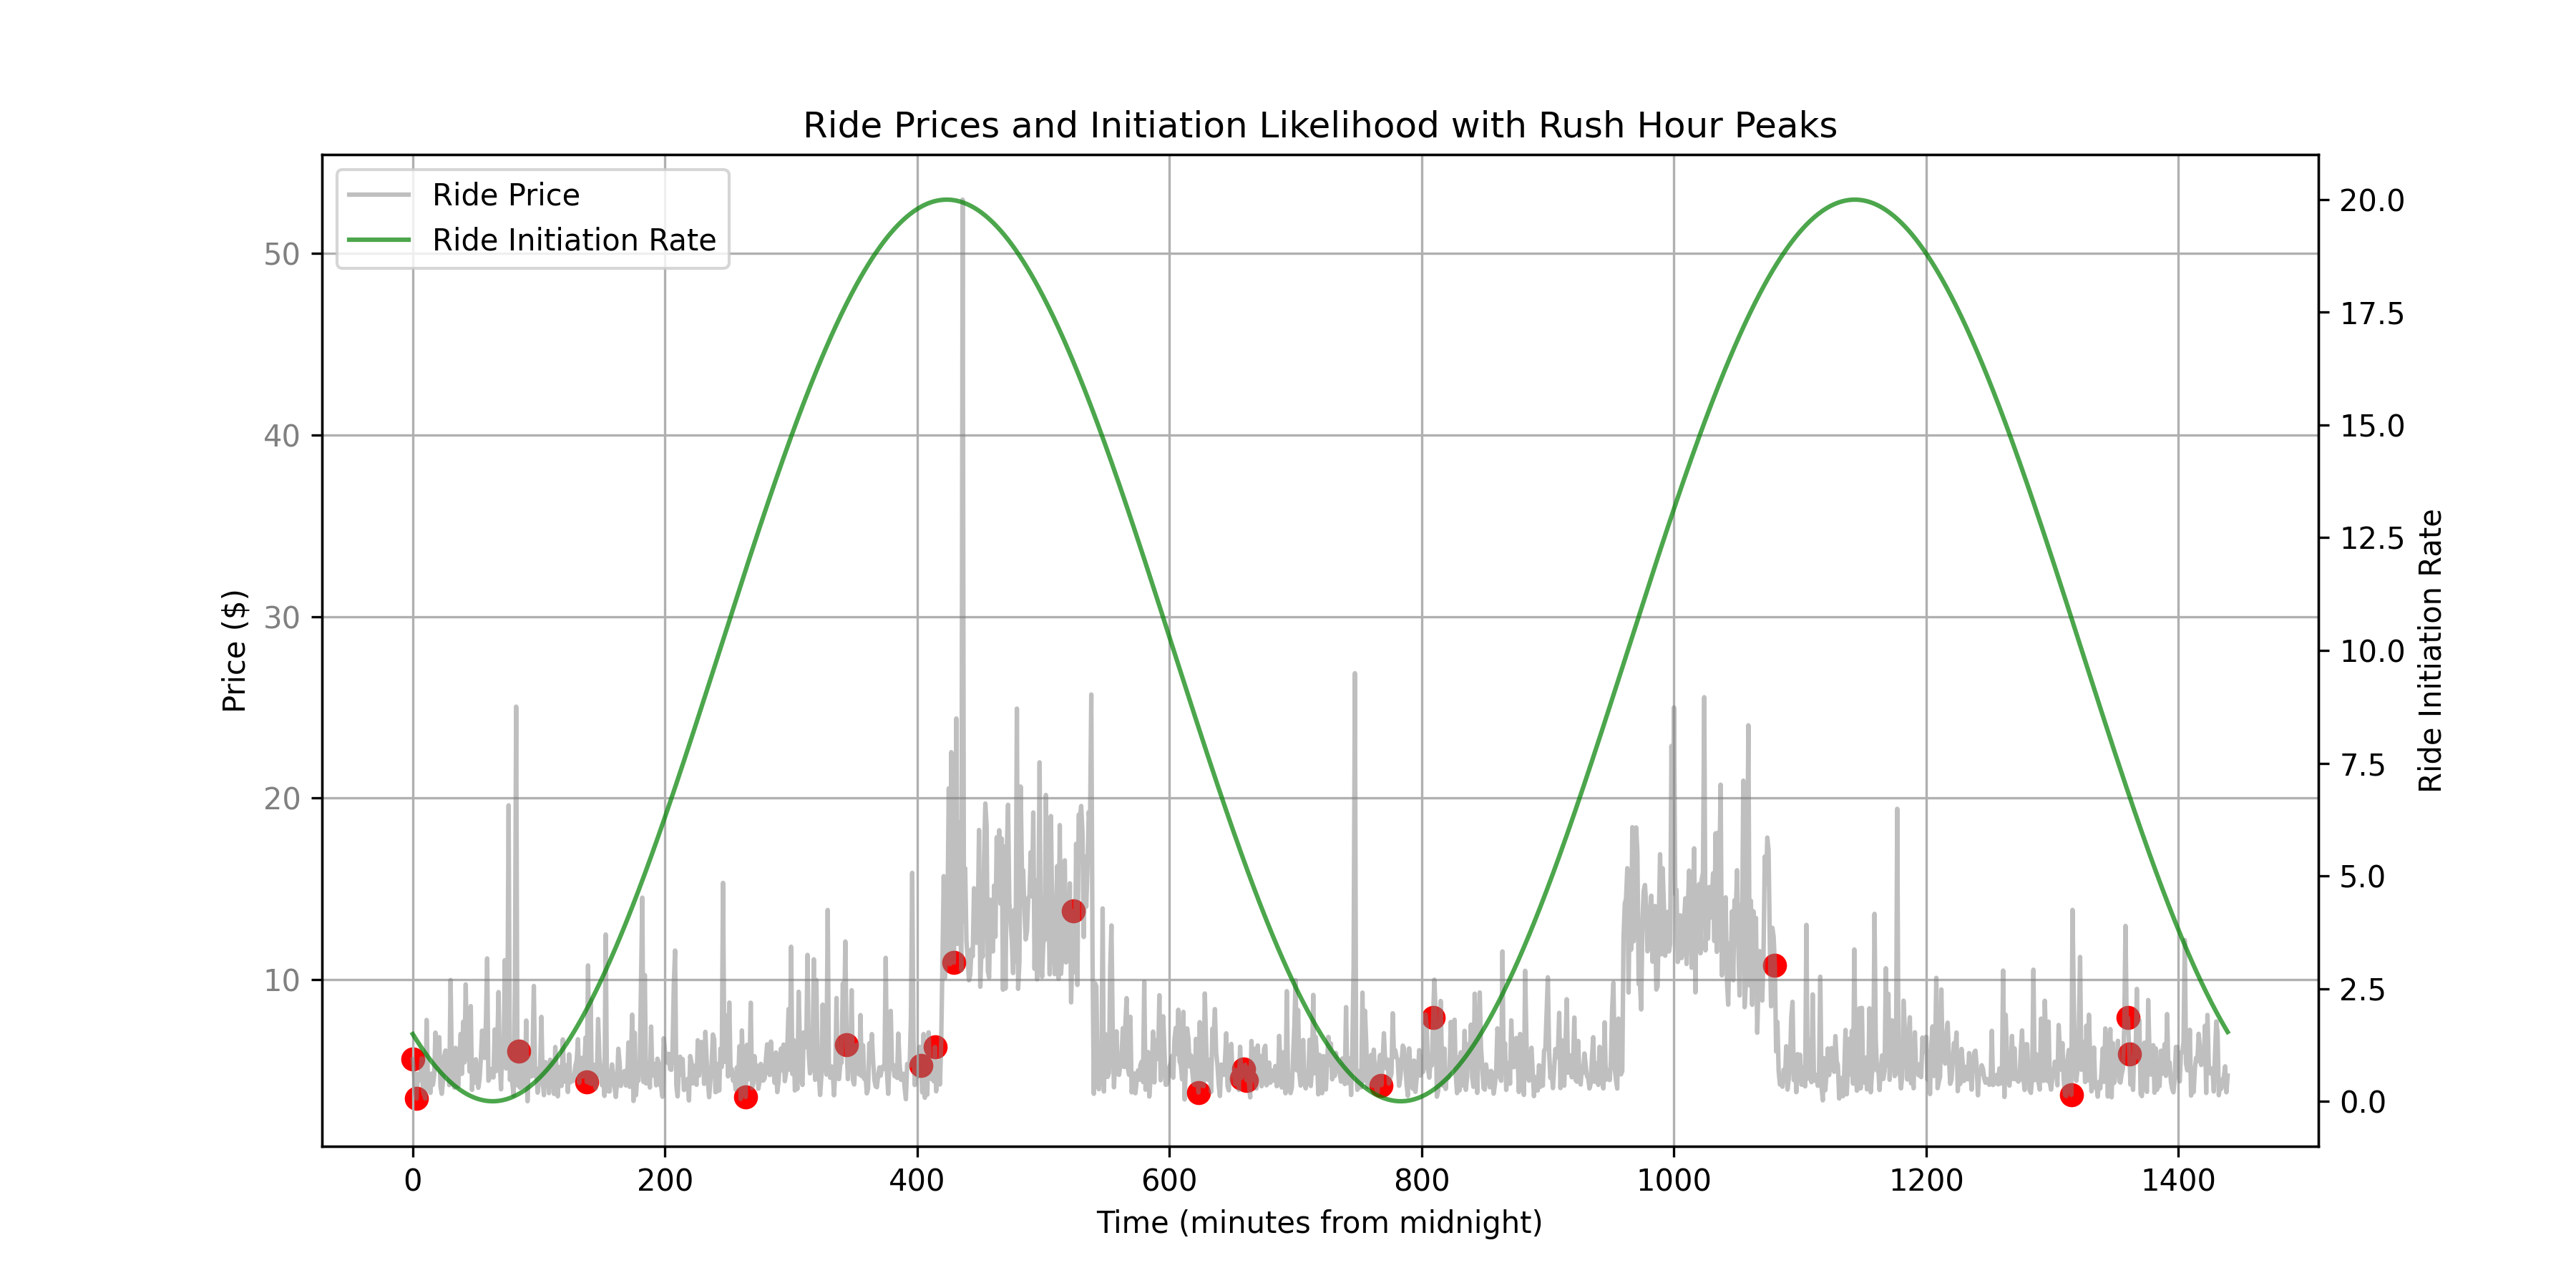
\includegraphics[width=0.9\textwidth]{img/ride_prices_plot.png}
    \caption{True price for rides starting at time $t$ over a fixed path $\path$. The price line is represent hypothetical rides, except at circled dots.
    }
    \label{fig:true-price}
\end{figure}

To determine the upfront premium for capping the price of a ride at $K$ over a period $[0,T]$, we need to consider the dynamics of ride initiation and pricing, as illustrated in Figure~\ref{fig:true-price}. Observed prices are represented by the round circles, while the grey line depicts a hypothetical price trajectory, highlighting the challenge that the true price distribution is only partially observed.

Calculating this premium requires computing (a) the ride initiation likelihood, (b) the probability that the uncapped price would have exceeded $K$, and (c) the present value of any potential price exceeding $K$. Available historical data on empirical ride initiation frequencies is statistically sufficient to compute (a). 
The sparsity of ride data necessitates a theoretical model of the price distribution to compute (b) adequately. Once (b) is determined, (c) can be computed using known financial tools. A generalized pricing distribution is, thus, at the core of achieving our objective of price capping.

\subsection{Outline}
We start with the necessary background material (Sec.~\ref{sec:background}), where we introduce the concept of metric graphs (Sec.~\ref{sec:metric-graph}) and cyclostationary processes on such graphs (Sec.~\ref{sec:cyclostationary}). With such info, we define the travel time process (Sec.~\ref{sec:traveltime-process}). Section~\ref{sec:pricing-main} establishes our first objective of characterizing the pricing equation in ride-share markets, its distribution, and the necessary assumptions to achieve our result. We solve, in Section~\ref{sec:upfront}, an analytical equation for up-front pricing of on-demand (instantaneous rides) that guarantees a fixed predetermined price. We do so for population and trip-specific rides, building on the work~\cite{elmasri2020predictive, woodard2017predicting} and establishing our second objective. Finally, we develop a more comprehensive framework for pricing complex transportation products, such as commuter rides, in Section~\ref{sec:complex-pricing}. We demonstrate our work in a case study in Section~\ref{sec:case-study}.

\subsection{Literature review}
\label{literature}
Previous research has shown that incorporating uncertainty into travel time estimates can lead to improved outcomes in ride-sharing systems, such as higher driver-rider match rates (up to 85\%) and lower average prices (up to 12\%) \citep{long2018ride}. These improvements can also positively impact other key system metrics, including reliability, service rate, utilization, and profitability \citep{li2021vehicle, li2022pricing,li2022ride}. Consequently, interest in understanding travel time uncertainty has been growing for practical reasons \citep{westgate2013travel,wang2019simple, hunter2009path,westgate2016large}.  Researchers have explored various approaches, ranging from models that estimate uncertainty from individual edges \citep{zheng2013urban,jenelius2013travel} to those that estimate route and travel uncertainty simultaneously \citep{westgate2013travel,wang2019simple, hunter2009path,westgate2016large}. With the increasing volume of collected GPS data, research has primarily focused on understanding the distribution of travel time through parametric methods \citep{woodard2017predicting,guo2012multistate,ma2017estimation,zhang2019novel} or by examining the limiting properties of stochastic and dynamical processes resembling real-world travel behaviour \cite{elmasri2020predictive, bolin2022gaussian}.

Recent progress has shown that deviations in travel time behave similarly to deviations from a normal distribution~\cite{elmasri2020predictive, woodard2017predicting}. Therefore, it is not surprising that regression-based models have shown promising results in travel time modelling \citep{westgate2016large, woodard2017predicting,budge2010empirical, westgate2013travel}. In particular,~\cite{elmasri2020predictive} have suggested a Gaussian form as a population-style distribution for travel time, where both the mean and variance scale with distance. For example, a \(N(n\mu, n\sigma^{2})\), where \(n\) is the number of road segments and \((\mu, \sigma^{2})\) are map- (possibly traffic time bin-) specific mean and variance constants. A similar distribution has been proposed for route-conditional travel time. 

For a survey of dynamical processes on networks (including transportation networks), see~\citet[ch. 11]{barrat2008dynamical}, for resent statistical work on the topic see~\citep{kolaczyk2014statistical, snijders2017modeling,burk2007beyond, britton2002bayesian,golightly2005bayesian, bolin2022gaussian}. 

Dynamic pricing is central to ride-sharing platforms\footnote{like Uber and Lyft}, enabling real-time price adjustments to balance supply and demand while maintaining service quality~\citep{banerjee2015pricing, yan2020dynamic}. Research shows that dynamic pricing increases driver availability, reduces peak-hour demand, and minimizes inefficient pickups~\citep{chen2015peeking, hall2015effects}. However, price volatility and fairness remain challenges, which have been partly addressed through strategies like time-based ride batching and dynamic waiting windows~\citep{yan2020dynamic}. Beyond dynamic pricing, there is growing interest in pricing more complex transportation products, such as commuter memberships. Most work in this area focuses on optimization methods for commuter ride-sharing~\citep{WANG2019390, MA2017345}. To the best of our knowledge, our work is the first to take a methodological approach to ride pricing.

\section{Background}\label{sec:background}
\subsection{Metric graphs}\label{sec:metric-graph}
A finite graph $\cG = (\cV, \cE)$ consists of a set of a finite set of vertices $\cV =\cbr{v_i}$ and a set $\cE = \cbr{e_j}$ of edges connecting the vertices. We write $u \sim v$ or $\rbr{u,v} \in E$  if $u$ and $v$ are connected with an with edge. We let $\cG$ be a direct graph, that is, $\rbr{u,v}$ represents and edge from $u$ to $v$. We call a graph $\cG$ a metric graph, if every edge $e$ is assigned a length $0< l_e< \infty$, and over $e$ it possible to assign a coordinate  $c \in [0, l_e]$ which increases in a specified (but otherwise arbitrary) direction along the edge. Since the length $l_e$ are assumed to be finite, this implies that the graph is compact. A point $s \in \cG$ is a position on an edge, i.e.~$s = (e, x)$, where $x \in [0, l_e]$. A path $\path = \pathseq{\pstart}{\pend} \in \cG$ is a sequence of edges $\rbr{e_1, \dots, e_n}$ where the path starts at point $\pstart \in e_1$ and ends at $\pend \in e_n$. A natural choice of metric for the graph is the shortest path distance, which for any two points in $\cG$, it is defined as the length of the shortest path in $\cG$ connecting the two. We denote this metric by $\delta(\cdot, \cdot)$ from now on. We provide a path conditional version of this distance metric as $\delta_\path(s) = \delta_\path(s, \pstart)$, for $s \in \path$, as the distance between points $s$ and the start of the path $\pstart$, over the the path. We further let $\delta_\path$ defines the whole distance of $\path$. Let $n_\path = \abr{\cbr{e : e \in \path}}$ be the number of edges of $\path$. We assume that the graph is connected, so that there is a path between all vertices. We define $\Pi(e_1, e_2)$ to be the set of all paths between edge $e_1$ and $e_2$, and similarly $\Pi(\pstart, \pend)$ be the set of all paths between points $\pstart, \pend \in \cG$. 
There is no unique way of defining process over graphs. This is a result of various way of defining the boundary condition (vertex condition), such as the Neumann-Kirchhoff condition, see~\citet[Eq~(1.4.4) and Them~1.4.4]{berkolaiko2013introduction}. In this work, we treat a path $\path = \pathseq{\pstart, e_1}{e_n,\pend}$, as an extended sequence of an uninterpreted edge, having the geometry
\[\sbr{0,\;  \delta(\pstart, e_1) + \sum_{e\in \path} l_e + \delta(e_n, \pend)}, \]
without introducing intermediate vertices at $l_e,$ $e \in \path$.


For every edge $e\in \cE$, a function $f_e \in L_2(e)$ if $f_e$ is square-intergrable over the edge $e$. We further define a function $f$ over $\cG$ as a collection of functions $f = \cbr{f_e}_{e \in cE} \in L_2(\cG)$ if $f_e \in L_2(e)$ for each $e \in \cE$. Tihs results in $L_2(\cG)$ being the direct sum over $L_2(e)$ as 
\[L_2(\cG) = \bigoplus_{e \in \cE} L_2(e). \]

We finally let $C(\cG) = \cbr{f \in L_2(\cG): f \text{ is continuous}}$ be the space of continuous functions on $\cG$. We define $\RR_+$ to be the positive part of the real line.

\subsection{Cyclostationary processes over metric graphs}\label{sec:cyclostationary}
We let $X=X(t, s)$, for every fixed time index $t \in \RR_+$ and point $s \in \cG$, be a 2nd order cyclostationary process in the wide sense. Here $X(t,s)$ is spatio-temporal process defined as
\begin{equation} \label{eq:speed}
X(t,s) = m(t, s) + \epsilon(t, s), \qquad t \in \RR_+, s \in \cG,
\end{equation}
where, in the temporal domain (holding the spatial fixed), for every $e \in \cE$ and $t, u \in \RR_+$, we have
\begin{subequations}
\label{eq:mean-covariance}
\begin{align}
    m(t, s) & =\EE[X(t,s)] = m(t + T_e, s), \label{eq:mean}\\
    \sigma^2(t, s) &= \EE[\epsilon^2(t,s)] = \sigma^2(t +T_e, s), \label{eq:variance}\\
    \varsigma(t, u, s) &= \EE[\epsilon(t,s)\epsilon(u, s)] = \varsigma(t +T_e, u+T_e, s) \label{eq:covariance},
\end{align}
\end{subequations}
where $T_e \in \RR_+$ is an absolute positive constant defining the temporal cycle of edge $e$. Here, $m(t,s), \sigma^2(t,s), \varsigma(t,u, s) \in C(\cG)$ (measurable functions over $\cG)$, and $\EE[\epsilon(t,s)]=0$ for all pairs $(t, s) \in \RR_+ \times \cG$.  We further let $\max_{e\in \cE} T_e \leq T_\cG < \infty$ be the global temporal cycle over $\cG$. That is, all equalities in~\eqref{eq:mean-covariance} apply when replacing $T_e$ by $T_\cG$. By definition of cyclostationarity, for come absolute constant $U_1>0$, we have
\[\abr{m(t,s)} + \abr{\sigma^2(t,s)} \leq \max_{u \in [0, T_\cG]}\cbr{m(u, s), \sigma^2(u, s)} \leq U_1,\]
for all $t\in \RR_+$, which is a stronger condition than the classical growth condition imposed on stochastic random variables, see~\citet[Thm.~5.2.1]{oksendal2013stochastic}. We further assume Lipschitz continuity in space and time as 
\begin{equation}\label{eq:lip-condition}
    \abr{m(t,x) - m(u, y)} + \abr{\sigma^2(t,x) - \sigma^2(u,y)} \leq C_2 \cbr{\abr{t-u} + \abr{x-y}},
\end{equation}
for $t, u \in \sbr{0, T_\cG}$, $x,y \in \cG$, and $C_2>0$ is an absolute constant.~\eqref{eq:lip-condition} results in spatial Lipschitz continuity when $t=u$, and temporal when $x=y$. 

We assume a conditional independence condition between space and time, that is is 
\[X(t, x) \perp X(t, y) \;\given\; t; \qquad x,y \in \cG, x\neq y.\] 

We define a ride on $\cG$ to be a the pair $(\rho, t)$, representing the path $\rho$ of the ride and the start time $t_2>0$.

%We further define the space of temporal marginal random variables as 
% \begin{equation}\label{eq:maringal-speed}
%     X_e(t) = \int_{s\in e} dX(t,s), \quad \text{for } e % \in E
% \end{equation}
% with temporal marginal mean and variance functions as 
%\[m_e(t) = \int_{s\in e} m_e(t, s)ds\qquad \sigma^2_e(t) = \int_{s\in e} \sigma^2(t,s)ds,\]
% where we equip $m_e$ and $\sigma_e$ with the subscript that indicates the marginal for edge $e$. %The spatial marginal mean and variance functions are \[m(s) = \int_{(0, C_s]} m_e(t, s)dt\qquad \tau^2(s) = \int_{(0, C_s]} \sigma^2(t,s)dt,\]
%where $C_s$ is the temporal length of the cycle at point $s$. 



% A sequence of random variables that exhibit such a form of serial dependency, 
% with variables far apart being nearly independent, is referred to as a {\it mixing } sequence. Different mixing types have been introduced in the literature. Each mixing type is associated with a separate coefficient assessing its strength~\citep{bradley2005}. The most general, in a sense implied by many other types, is called \(\alpha\){\it -mixing} (strongly mixing), which is defined below.

% \begin{definition}[\citep{rosenblatt1956central}] \label{def:alpha-mixing} Let $(X_k, k \in \Z)$ be a sequence of random variables defined on the probability space $(\Omega, \F, P)$. Define the $\sigma$-algebra $\F_a^b$ as
% \(\F_a^b = \sigma(X_k, a\leq k \leq b, k \in \Z)\), \(1 \leq a \leq b\leq \infty.\)
% For each $n\geq1$ define the measure of dependence
% \begin{equation}\label{eq:alpha-mixing}
%     \alpha(n)= \sup_{k \geq 1}\sup_{A \in \F_1^k, B \in \F_{k+n}^\infty} |P(A \cap B) - P(A)P(B)|.
% \end{equation}
% If $\alpha(n) \rightarrow 0$ as $n\rightarrow \infty$, then $(X_k, k \in \Z)$ is said to be {\it $\alpha$-mixing}.
% \end{definition}

% Since \(X(t,s)\), for\(t>0, s \in \RR^2\), are not strictly stationary (meaning that they do not have a time-invariant distribution), we require an extra mixing condition that is slightly stronger than the maximal correlation coefficient (defined as \(\rho(n)\) in \cite{bradley2005}) and implies it, which is related to mixing of interlaced sets.
% \begin{definition} \label{def:rho-mixing} Following 
% Definition 
% \ref{def:alpha-mixing}, let \(\F_{A} =\sigma(X_{i}, i \in A)\) for any non-empty set \(A \subset \Z\). Define the dependency measure
% \begin{equation}
%   \label{eq:rho-mixing}
%   \trho (n)= \sup_{A, B}\sup_{f,g} |\Corr(f,g)|, \quad  f \in \L^{2}(\F_{A}),\; g \in \L^{2}(\F_{B}), \min_{i\in A,j\in B }|i-j| \geq n,
% \end{equation}
% where \(\L^{2}(\F_{A})\) denotes the space of square-integrable \(\F_{A}\) random variables, and the supremum is over all disjoint non-empty sets \(A, B \in \Z\).
% \end{definition}
\subsection{Travel time process}\label{sec:traveltime-process}
We first define a transportation network $\cN = (\cG, X)$ to be a metric graph $\cG$ equipped with wide-sense cyclostationary process $X(t, s)$, $t \in \RR_+$ and $s \in \cG$. Travel time over a path $\path = \pathseq{\pstart}{\pend} \in \cG$ can be directly computed as the stochastic integral 
\begin{equation}
    \label{eq:traveltime-process}
\T_\path = \int_\path X(\T_s, s)ds = \int_\path m(\T_s, s)ds + \int_{\path} \epsilon(\T_s,s)ds, \quad \T_\pstart = 0
\end{equation}
where $\int_\path$ represent integration over the predetermined path $\path$, with $s \in \path$ being a point over the path. Here, $\T_s, s \in \path$ defines the travel time up to location $s$ on $\path$, such that the travel time at the start point $\pstart$, $\T_\pstart =0$. ~\cite{elmasri2020predictive} approximated the integral~\eqref{eq:traveltime-process} by a discrete version $\T_\path^d$, as 
\[\T^d_\path = \sum_{e \in \path} m_e(\tau_e) + \epsilon_e(\tau_e), \]
where 
\begin{equation}\label{eq:marginals}
    m_e(t) = \int_e m(t,s)ds, \quad \sigma^2_e(t) = \int_e \sigma^2(t,s)ds, \quad \epsilon_e(t) = \int_e \epsilon(t,s)ds,
\end{equation}
for $t \in \RR_+$.~\eqref{eq:marginals} are the spatial marginals over $X(t,s)$ defined in~\eqref{eq:speed}. We have implicitly assumed that all edges are traversed in $\T_\path^d$, and that $\T_\path^d$ is defined on a transportation network $\cN^d$ defined by the marginals of $X$, such that $\cN^d = (\cG, X^d)$, and $X^d = \cbr{X_e(t)}_{e \in \cE}$, where $X_e(t) = \int_e X(t,s)ds$. The following lemma is an adaptation of \citet[Lem~6, Them.~6]{elmasri2020predictive} that characterize the asymptotic distribution of $\T_\path^d$. 

\begin{lemma}[Population distribution~\cite{elmasri2020predictive}] \label{lem:population-distribution}Consider $\path$ as a random walk over the $\cN^d$ and let $\tau = \cbr{\tau_e}_{e \in \path}$ be the random arrival times over edges of the walk $\path$. Let  $\tau$ be sufficiently mixing\footnote{at least $\rho$-mixing, see~\cite{bradley2005} and \citet[Lem.~5,6]{elmasri2020predictive}}. Then as the number of edges in $\path$ grow to infinity (i.e.~$n_\path \to \infty)$, we have
\begin{subequations}\label{eq:population-asymp-dist}
\begin{align}
    n_\path^{-1}\T^d_\path &\stackrel{\text{a.s.}}{\to} \mu \\
    n_\path^{-1/2}(\T^d_\path - n_\path\mu) &\stackrel{d}{\to} N(0,\sigma^2), \label{eq:population-distribution}
\end{align}
\end{subequations}
where $\mu$ and $\sigma^2$ are absolute positive constants that are independent of initial conditions and of $\path$. 
\end{lemma}

The result in~\eqref{eq:population-asymp-dist} suggest that deviations of $\T_\path$ around the average travel time per edge $\mu$, normalized by $\sqrt{n_\path}$, resemble independent samples from a normal distribution, with variance that is independent of the route. However,~\eqref{eq:population-asymp-dist} is an asymptotic distribution over a population of rides in a system. That is for an arbitrary ride from a population of rides, the probability it arrives before $n_\path\mu$ is $1/2$. For a specific ride, say $(\rho_i, t_2)$, this probability can be significantly different if $\T_{\path_i}$ has not reached the asymptotic distribution. The following lemma is an adaptation of~\citet[Thm.~7]{elmasri2020predictive} that characterized the distribution of travel time for a specific ride. First, we define a deterministic mean and covariance sequences for a ride over $\path=\pathseq{e_1}{e_{n_\path}}$, starting at $t_1\in \RR_+$, as
\begin{subequations}\label{eq:mean-covariance-seq}
    \begin{align}
        t_{i+1} &= t_{i} + m_{e_i}(t_i), \quad i \in \cbr{2,\dots, n_\path},\\
        \mu_\path &= \sum_{i =1}^{n_\path} m_{e_i}(t_i), \\
        \sigma^2_\path &= \sum_{i=1}^{n_\path} \sigma^2_{e_i}(t_i) + 2 \xi \sum_{i=2}^{n_\path}\sigma_{e_i}(t_i)\sigma_{e_{i-1}}(t_{i-1}),
    \end{align}
\end{subequations}
for some absolute constant $\xi$. Here, $m_e$ and $\sigma^2_e$ are the spatial marginals defined in~\eqref{eq:marginals}. 

\begin{lemma}[Route-predictive distribution, Thm.~6 in~\cite{elmasri2020predictive}] \label{lem:route-predictive} Under the conditions of Lemma~\ref{lem:population-distribution}, for an arbitrary start time $t_0 \in \RR_+$, given a path $\path=\pathseq{e_1}{e_{n_\path}} \in \cG$, we have 
\begin{equation}\label{eq:route-distribution}
    \sigma^{-1}_{\path} \rbr{\T^d_\path - \mu_\path} \stackrel{d}{\to} N(0, \eta), \quad \text{as  } n_\path \to \infty,
\end{equation}
where $\eta$ is a strictly positive constant that is independent from initial conditions, and $\sigma^2_\path $, $\mu_\path$ are defined in~\eqref{eq:mean-covariance-seq}. 
\end{lemma}

The result of Lemma~\ref{lem:route-predictive}, although still suggests approximate normality of travel time distribution, it integrates route-specific information in the mean and covariance functions~\eqref{eq:mean-covariance-seq} to better approximate this distribution. As shown in~\citet[Fig.~3]{elmasri2020predictive}, the approximation in~\eqref{eq:route-distribution} can achieve significant accuracy when compared to~\eqref{eq:population-distribution}. 

Working with $\T_\path$ in~\eqref{eq:traveltime-process} directly is challenging, since the distribution of $\epsilon$ is not well understood. Every edge $e \in \path$ can influence $\T_\path$ differently, depending on the cyclostationarity pattern of the variance $\sigma(t,s)$ and the actual error distribution. 

To overcome such challenges, we rely on the results in Lemma~\ref{lem:population-distribution} and~\ref{lem:route-predictive}. The mean and covariance functionals $\mu(t,s)$, $\sigma(t,s)$ in~\eqref{eq:mean-covariance} define manifolds over the graph $\cG$. Using the asymptotic normality of travel and those functionals, we redefine travel time as the stochastic process, initiated at $\pstart=0$, as
\begin{equation}\label{eq:stochastic-travel-time}
    d\T_{s} = \alpha(\T_{s}, s)ds+ \beta(\T_{s}, s)dB_s,\qquad \T_{\pstart} = 0,   \quad s \in \path,
\end{equation}
where $B_s$ is Brownian process.~\eqref{eq:stochastic-travel-time} suggests that travel time over a route $\path$ behaves like an arithmetic Brownian motion on the spatial domain, having the expectation and variance as 
\[\EE[\T_s] = \int_\path \alpha(\T_s,s)ds \quad \Var[\T_s]  = \int_\path \beta^2(\T_s, s)ds, \quad s \in \path,\]
where the variance follows by the assumption that $B^2(t,s)$ is bounded, and thus by the Itô isometry property \citet[Lem.~3.1.5]{oksendal2013stochastic}, we have $\EE\rbr{\int_\path \beta(\T_s, s)dB_s}^2 = \int_\path \beta^2(\T_s,s)ds$. 

Finally, to adapt $\T_\path$ to the population version in Lemma~\ref{lem:population-distribution} and the route-specific version in Lemma~\ref{lem:route-predictive}, we let $\alpha$ and $\beta$ be 

\begin{equation}\label{eq:mean-variance-sde}
    \alpha(t,s) = 
    \begin{cases}
        \mu & \text{population} \\
        m(t,s) & \text{route-specific}
    \end{cases}
    \qquad 
    \beta(t,s) = 
    \begin{cases}
        \sigma & \text{population}        \\
        \sqrt{\eta}\sigma(t,s) & \text{route-specific},
    \end{cases}
\end{equation}
where $m(t,s)$ and $\sigma(t,s)$ are as defined in~\eqref{eq:mean-covariance} and $\eta$ is a universal parameter that is estimated from data and accounts for residual error. 


\section{Assumptions in ride-share markets}
In traditional pricing theory, three primary approaches dominate: cost-based, market-based (competition-driven), and value-based pricing \cite{phillips2021pricing}. This study proposes a pricing policy for a ride-sharing platform that is entirely cost-based, independent of real-time supply-demand dynamics. Unlike prior research focusing on matching algorithms or market-based pricing (see \ref{literature}), we assume prices are determined by equation \eqref{eq:price}. The goal is to recover operational costs based on traffic and route assumptions, rather than to maximize profit. We operate in a monopoly market, assuming all ride requests are satisfied immediately (no unmatched requests).


Our analysis focuses on the pricing mechanism from the moment a rider submits a request until the driver completes the trip. To isolate the pricing dynamics, we make the following   assumptions to focus  on the pricing mechanism:
\begin{enumerate}[label={(A$_{\arabic*}$)}, ref={(A$_{\arabic*}$)}]  
	\label{monopoly}
	\item Once a rider submits a request, they do not cancel, and a driver accepts and completes the trip immediately, with no rematching or wait time.
	
	\item The platform is a monopolist with full pricing power, facing no competition or alternative transportation options for riders.
	
	\item For every ride request, an available driver exists to fulfill it within a finite time.
	
	\item Both riders and drivers are non-strategic and price-insensitive beyond the modelled price; they do not respond to changes in market conditions or alternative routing options.
	
	\item No ride-specific information (e.g., route, traffic, or weather) is known at the time of membership subscription. (Once  they hold the membership, they may abuse it.)
\end{enumerate}


Moreover, we assume a frictionless environment:
\begin{enumerate}[label={(B$_{\arabic*}$)}, ref={(B$_{\arabic*}$)}]  
	\item The risk-free interest rate $r$ is constant over time and known. \label{frictionless}
	
	
	\item  There are no transaction costs, taxes, or additional platform fees beyond the modeled price.
	
	
	Under our assumptions, riders are price-insensitive but may increase usage in response to external conditions (i.e, abuse  as mentioned in section \ref{membership_abuse}).  This setup reflects a monopoly market with non-strategic supply, where the platform acts as the sole decision-maker, and the customer accepts the offered price without negotiation or cancellation. The pricing method is not explicitly adjusted based on real-time fluctuations in driver supply or rider demand. 
	
Our objective is to propose a cost-based pricing method and evaluate its stability and volatility under dynamic conditions, such as varying traffic or membership abuse, without modeling equilibrium outcomes in a two-sided market. 	We explicitly exclude the matching process, strategic driver behavior, and real-time supply-demand equilibrium mechanisms from our analysis.

While dynamic pricing based on real-time demand and supply can, in theory, maximize revenue, it is often operationally costly and computationally intensive. In practice, rider behavior is highly unpredictable and sensitive to wait time and price fluctuations, leading to instability. The tradeoff in our method  is a potential loss in revenue in exchange for greater pricing stability and predictability.
\end{enumerate}

\section{Pricing equation in ride-share markets}\label{sec:pricing-main}
Ride pricing is determined by three constant factors predefined by the service provider. A fixed price $C_0$ (starting price), a cost for a unit of time $C_1$, and a cost for a unit of distance $C_2$. Let $P_\path(s, t)$ be the price of a ride that starts at time $t>0$, over the route $\path$, and at location $s \in \path$, that is
\begin{equation}\label{eq:price}
    P_\path(s, t) = C_0 + C_1\T_s(t) + C_2 \delta_\path(s), \qquad s \in \path, 
\end{equation}
where $\T_s(t) = \T_{\path(s)}(t)$ is the travel time up to point $s \in \path$ and starting at time $t>0$ and $\delta_\path(s) = \delta(s,\pstart)$ is the length of the path $\path$ up to point $s$. To simplify notations, we will drop the $(t)$ from $\T_s(t)$, since the start time defined in the pricing function $P_\path(s, t)$. The base price is determined at the start point $\pstart \in \path$, that is 
\[P_{\pstart}(\pstart, t) = C_0, \quad \text{for all } t > 0, \]
and the final price is determined at the destination point $\pend$, and arrival time $t_2$, as
\[P_\path(\pend, t) = C_0 + C_1\rbr{t_2 - t} + C_2\delta_\path.\]

Here,  $\T_{\path(\pend)} = t_2 -t$, an actual realization. Otherwise, for any point $s \in \path \setminus \cbr{\pstart, \pend}$, the price equation~\eqref{eq:price} is a random variable determined by $\T_s(t)$. Moreover, for any two points $s_1, s_2 \in \path$, if $s_2$ is further along $\path$ than $s_2$ (i.e.~$\delta_\path(s_1) \leq \delta_\path(s_2)$), then 
\[P_\path(s_2,t) \geq P_\path(s_1,t).\]

Such inequality in the time domain is not true, that is $P_\path(s, t_1)$ is not necessary less than $P_\path(s,t_0)$ for $t_1 < t_0$, and $s \in \path$. The price equation~\eqref{eq:price} is, thus, composed of three components: (i) the fixed price $P_\path(0,0) = C_0$, (ii) the incremental price $C_2\delta_\path(s)$, and (iii) the variable price $C_1\T_s, s \in \path$. In this sense, the true price of a ride over $\rbr{t,\path}$ that arrived at $\T_\path = t_2 - t$, is 
 \begin{equation}\label{eq:true-price}
    P_\path(\pend, t) = C_0 + C_1(t_{0} -t) + C_2 \delta_\path,
 \end{equation}

 If the realization is not yet observed, then the present value of the ride price at start location $\pstart$ is a random variable having the expectation
\begin{equation}\label{eq:predicted-price}
    P_\path(\pstart, t) = \EE\sbr{P_\path(\pend, t)}= C_0 + C_1\EE\sbr{\T_\path} + C_2 \delta_\path,
 \end{equation}

In~\eqref{eq:predicted-price}, the expectation is taken over all possible realization of $\T_\path$, without accounting for the value of money. For example, having the option to allocate the cost of the ride, say $K$, to an investment vehicle with a risk-free annualized interest rate $i$, would earn $Ke^{i\T_\path}$ by the time the ride arrives. In this sense, the price of a ride $(t, \path)$ at the start location $\pstart$ is 
\[P_\path(\pstart, t) = \EE\sbr{e^{-i\T_\path} P_\path(\pend, t)}. \]

Adjusting for the value of money is mostly mathematical exercise, since in most real-world applications, arrival times are within minutes. Exceptions exists, for example cargo and fright, which can take last weeks. Such adjustment can be useful for schedules of rides or membership pricing as shown in later sections.

Finally, the present value of the pricing formula can be extended to route unconditional pricing through expectations. Given the set of all path $\Pi\rbr{\pstart, \pend}$  between origin-destination pair $(\pstart, \pend)$. The price of the ride  $(t, \pstart, \pend)$ is
\[P_{\rbr{\pstart, \pend}}(\pstart, t) = \EE\sbr{e^{-i\T_{\path_k}}P_{\path_k}(\pend, t)},\qquad \path_k \sim \Pi(\pstart, \pend),\]
where the expectation is taken over the uniform distribution of routes, and travel time. A discrete probability measure can be applied on the set $\Pi$, for a non-uniform distribution.


\subsection{Up-front pricing} \label{sec:upfront}
Up-front pricing, a popular initiative by ride-share providers, promises a price $K$ at the request time $t$ for a ride over the path $\path$ starting at location and time $(\pstart, t_0)$, $t_0\geq t$, and potentially ending a location and time $(\pend, t_1)$. When $t_0=t$, we call this an on-demand ride, otherwise this is a scheduled ride. The progression if a ride request is shown in Figure~\ref{fig:ride-time}. 

\begin{figure}[th!]
\centering
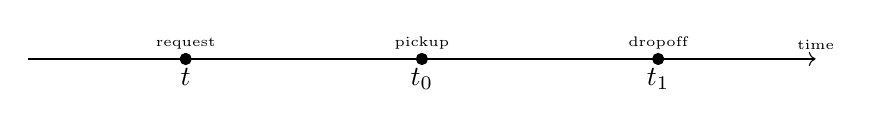
\begin{tikzpicture}
  \draw[->] (0,0) -- (10,0) node[above]{\tiny time}; % Arrow line
  \filldraw[black] (2,0) circle (2pt) node[below] {$t$} node[above] {\tiny request};
  \filldraw[black] (5,0) circle (2pt) node[below] {$t_0$} node[above] {\tiny pickup};
  \filldraw[black] (8,0) circle (2pt) node[below] {$t_1$} node[above] {\tiny dropoff};
\end{tikzpicture}
\caption{Time progression of a rides request, pickup and dropoff.}
\label{fig:ride-time}
\end{figure}

The upfront price $K$ is guaranteed unless the realized price $P_\path(\pend, t_1)$ does not exceed a cutoff threshold, which is often defined as a percentage of the upfront price, say $Ke^\zeta$, for a predefined constant $\zeta \in \RR_+$ predefined\footnote{a link to pricing policy to be added}. Under Assumption~\ref{frictionless}, a request if accepted is always fulfilled. let $R(t_1, t_0, \path, K)$ be the cost of this liability at the time of execution (i.e.~the arrival time $t_1$), defined as 
\begin{equation}\label{eq:ride-cost}
    R(t_1, t_0, \path, K) = \rbr{P_\path(\pend, t_1) - K}^+\one_{\cbr{P_\path(\pend, t_1) \geq Ke^\zeta}}. 
\end{equation}

In this sense, the final price charged to the customer at time $t_1$ is
\begin{equation}\label{eq:charged-upfront-price}
K + R(t_1, t_0, \path, K) = 
\begin{cases} 
P_\path(\pend, t_1) & \text{if } Ke^\zeta \leq P_\path(\pend, t_1) \\
K & \text{otherwise}.
\end{cases}
\end{equation}
It is clear from~\eqref{eq:ride-cost} that for promised ride price $K_1 \geq K_2$, we have 
\[R(t_1, t_0, \path, K_1) \leq R(t_1, t_0,, \path, K_2).\]

Oftentimes rideshare providers do not explicitly estimate the cost of such a guarantee at time the request time $t$, that is $R(t, t_0, \path, K)$. Instead, consumers are only charged $K\$$ at time $t_0$. At arrival time $t_1$, the price is adjusted according to~\eqref{eq:charged-upfront-price}.  

Under Assumptions~\ref{monopoly}, we model the travel time along the path $\path = \pathseq{\pstart}{\pend}$ as an asymptotic stochastic dynamic governed by the partial differential equation~\eqref{eq:stochastic-travel-time}. The price of the guarantee~\eqref{eq:ride-cost} at request time $t$ is then given by:
\begin{equation}\label{eq:european-knock-in}
\begin{aligned}
 R(t,t_0, \rho, K) &= \EE\sbr{e^{-r(t_0-t)}R(t_1,t_0, \path, K)} \\
  &= \EE\sbr{e^{-r(t_0-t) -r\T_\path}\rbr{P_\path(\pend, t_1) - K}^+ \one_{\cbr{P_\path(\pend, t_1) \geq Ke^\zeta}}}  \\
  &=e^{-r(t_0-t)} e^{-rd_7}\sbr{\cbr{d_0 - rC_1d_1^2- K}\cbr{1-\Phi\rbr{d_5}} + C_1d_1 \phi(d_5)} \\
    \end{aligned}
\end{equation}
where 
\begin{align*}
    d_0 & = C_0 + C_1\EE[\T_\path] + C_2\delta_\path\\ 
    d_1 &= \cbr{\Var[\T_\path]}^{1/2} \\
    d_4 &= \frac{Ke^\zeta -d_0}{C_1d_1} \\
    d_5 &= d_4 + rd_1\\
    d_7 &= \EE[\T_\path] - rd_1^2/2
\end{align*}

When $r=0$, the solution to \eqref{eq:european-knock-in} simplifies to 
\[ R(t,t_0, \rho, K) = (d_0-K)\cbr{1- \Phi(d_5)} + C_1d_1\phi(d_5).\]

Further if $\zeta=0$, as there is no minimum threshold for the guarantee, we have 
\[ R(t,t_0, \rho, K) = (d_0-K)\cbr{1- \Phi(d_8)} + C_1d_1\phi(d_8),\]
where
\[d_8 = \frac{K - d_0}{C_1d_1}.\]

The next section introduces more complex pricing structures with unknown routes and start times, and packages them into membership offering. 

\subsection{Pricing complex products}\label{sec:complex-pricing}
Pricing of on-demand single rides in Section~\ref{sec:pricing-main} is done under the simplest case of known (route, start time)$=(\path, t_0)$. We vary these two quantities by generalizing from a known fixed route to only the (start, end) $=\rbr{\pstart, \pend}$ locations are known, and then an unknown start time. Summarized in three pricing products
\begin{enumerate}[label={(P$_{\arabic*})$}, ref={(P$_{\arabic*}$)}] 
    \item On-demand. An instantaneous ride request to go from  $\pstart$ to $\pend$ in $\cG$ over the route $\path$. \label{on-demand}
    \item Scheduled. A ride request to go from $\pstart$ to $\pend$ in $\cG$ at a future time $t$. \label{scheduled}
    \item Membership. An option to request up to $M$ rides within a pacified time interval, $T_M \in \RR_+$, at a predetermined price $K$. Such rides can be (but not necessarily) conditioned over fixed hours and locations.  \label{membership}
\end{enumerate}

Computing an accurate upfront price--paid at the time of request or subscription--is the central challenge in three scenarios of increasing complexity:~\ref{on-demand}, \ref{scheduled}, and \ref{membership}. The information available at the pricing time diminishes with each case. In the on-demand scenario \ref{on-demand}, both the route's start/end points and the real-time network dynamics are known. For a scheduled ride~\ref{scheduled}, only the start/end locations are known, requiring a forecast of network dynamics. Finally, under a membership plan~\ref{membership}, no details are known at the pricing stage, and the ride itself is elective. 

The premium price of the on-demand~\ref{on-demand} scenario is defined in~\eqref{eq:european-knock-in}. Recall that $\Pi(\pstart, \pend)$ is the set of routes between any two points, $\pstart$ and $\pend$. Let $\pi(\path)$ be the likelihood of route $\path$ in $\Pi(\pstart, \pend)$. If a uniform distribution is desired, then $\pi(\path) \propto 1/\abr{\Pi(\pstart, \pend)}$. $\pi(\path)$ can (not necessarily) time dependent. The premium price of the scheduled ride~\ref{scheduled} requested time $t$ for (start time, start location, end location) = $(t_0, \pstart, \pend)$ is
\begin{equation}
\begin{aligned}\label{eq:scheduled-price}
    \scheduled(t, t_0, K) & = 
\sum_{\path_i \in \Pi\rbr{\pstart, \pend}} R(t, t_0, \path_i, K)\pi(\path_i) \\
& = \sum_{\path_i \in \Pi\rbr{\pstart, \pend}} \EE\sbr{e^{-r(t_0-t + \T_{\path_i})}R(t_1, t_0, \path, K)}\pi(\path_i) \\
 & = \sum_{\path_i \in \Pi\rbr{\pstart, \pend}} \EE\sbr{\EE \sbr{e^{-r(t_0-t) - r\T_{\path_i}}R(t_1, t_0, \path, K)\given t_0}}\pi(\path_i) \\
& = e^{-r(t_0-t)} \sum_{\path_i \in \Pi\rbr{\pstart, \pend}} \EE\sbr{e^{-r\T_{\path_i}}R(t_1, t_0, \path, K)}\pi(\path_i).
\end{aligned}
\end{equation}

The pricing in~\eqref{eq:scheduled-price} occurs by averaging over all routes between $\pstart$ and $\pend$, hence the notation $\bar R$. In the same spirit, let $\pi(t)$ be the distribution of pickup times on the interval $T_R$. The price guarantee of a membership~\ref{membership} purchased at time $t$ of $M$ rides on the interval ride~\ref{scheduled}, for fixed price $K$, is
\begin{equation}\label{eq:membership-price}
\begin{aligned}
    \memebership(t, M) & = M
    \sum_{t_0 \in [0, T_R]} 
    \sum_{\path_i \in \Pi\rbr{\pstart, \pend}} 
    R\rbr{t_0, t_0, \path_i, K_{\path_i}}
    \pi(t_0) \pi(\path_i), \\
    & = M \sum_{t_0 \in T_R} e^{-r\rbr{t_0 - t}}
    \sum_{\path_i \in \Pi\rbr{\pstart, \pend}} 
    R\rbr{t_0, t_0, \path_i, K}
    \pi(t_0) \pi(\path_i), \\
      & = M \sum_{t_0 \in  T_R} e^{-r\rbr{t_0 - t}}
    \sum_{\path_i \in \Pi\rbr{\pstart, \pend}} 
    \EE\sbr{e^{-r\T_{\path_i}}R\rbr{ t_1, t_0, \path_i, K}}
    \pi(t_0) \pi(\path_i), \\
    & = M \sum_{t_0 \in T_R} e^{-r\rbr{t_0 - t}} \scheduled\rbr{t_0, t_0, K}   \pi(t_0),
\end{aligned}
\end{equation}
where $\scheduled$ follows from~\eqref{eq:scheduled-price}. To validate our method, the next section develops a statistical sampling methods for routes and travel time. 

\section{Statistical sampling of travel times and routes}\label{sec:sampler}
To simulate alternative routes to a realized trip, we develop a statistical approach for trip sampling, and demonstrate its statistical fidelity. Given a trip (route, start time)$=(\path, t_2)$, we alternative routes, then we sample travel times.
\subsection{Route sampling}\label{sec:route sampling}
When all traffic states of the graph is observed, routing-finding algorithm, such as the one proposed by~\cite{1970algorithm}, can be used to list all routes from two points ($e_1, e_n)$ on the $\cG$ at the desired start time $t_2$. Marrying this route sampling approach to reality is intuitive, but not always possible. Existing traffic data do not cover all states of the graph.  Our objective is propose a sample method that provide statistically equivalent routes, that are graph-invariant for all triplet (start location, end location, start time) = ($e_1, e_n, t_2)$. 

Given a route $\langle e_1, e_2 \dots, e_n \rangle$, first, we match edges $\times$ time bins using a mean matching method. or each edge $e \in E$ and time bin $b \in B$, let $n_{e,b}$ be the sample size used to calculate the sample mean $\hatm_e(t_b)$ and variance $\hatsigma_e(t_b)$. We define statistically equivalent edges by the difference between their means, as 
\begin{equation}\label{eq:similar-edges}
E_{e, b}(\zeta) =
\cbr{
    \rbr{e', b'} \in E \times B:
    {\frac
    {\abr{\hatm_e\rbr{b} - \hatm_{e'}\rbr{b'}}}
    {\sqrt{\frac
        {\hatsigma_e(b)}
        {n_{e,b}} 
        +
        \frac
        {\hatsigma_{e'}(b')}
        {n_{e',b'} }
    }} \leq \zeta
    }
    } 
\end{equation}

The set in~\eqref{eq:similar-edges} is constructed using simultaneous t-tests, with unequal variance and sample size, on the hypothesis that the two edges $e, e'$ have equivalent means under the time bins $b, b'$. The critical value $\zeta$ can be chosen to achieve a $(1-\beta)100\%$, $\beta \in (0, 1)$ level of significance of the Student's t distribution with  degrees of freedom following the Welch–Satterthwaite equation~\citep{satterthwaite1946approximate,welch1947generalization}, as
\[
\textsf{degrees of freedom} = 
\frac{
\rbr{{\frac
        {\hatsigma_e(b)}
        {n_{e,b}} +
    \frac
        {\hatsigma_{e'}(b')}
        {n_{e',b'} }
    }}^2
}{
 \frac{\rbr{\hatsigma_e(b)/ n_{e,b}}^2}{ n_{e,b}-1} 
 + 
  \frac{\rbr{\hatsigma_{e'}(b')/ n_{e',b'}}^2}{ n_{e',b'}-1}
}
\]

Second, we randomize the length of the sampled route using a normal distribution centered at the number of edges $n$ of a given realized route. This results in a route sampling process as
\begin{equation} \label{eq:route_sampling}
\begin{aligned}
    t_0 & \sim \textsf{given start time} \\
    \path = \langle e_1, e_2 \dots, e_n \rangle & \sim \textsf{given route } \path \\
    E_{\path} &= \cbr{E_{e, b}: (e,b) \in \path }\\
    n'& \sim {\lfloor}\textsf{Normal}\sbr{n, \tau}{\rfloor}\\
    \path' = \langle e'_1, e_2 \dots, e'_{n'} \rangle & \sim \textsf{Uniform}\sbr{E_\path}. 
\end{aligned}
\end{equation}

Here $ {\lfloor} Z {\rfloor}$ represent the integer floor of a positive variable $Z$.   

\subsection{Travel time sampling}\label{sec:travel time sampling}
We define $B$ to be the set of time bins of the data, for example, EveningRush, WeekDay, MorningRush, EveningNight, and WeekendDay, used in~\cite{elmasri2020predictive}. For every edge $e \in \cG$, let $\hatm_e(t_b)$ and $\hatsd_e(t_b)$ be the sample average speed and standard deviation of duration to travel $\T_e$, respectively. Here $t_b \in B$, meaning, i.e.~a time bin. We reserve the notation $t_b$ to represent the time bin $t$ falls into. This results in $\abr{E} \times \abr{B}$ number of traffic states in $\cG$. 

Following the simple auto-regressive structure and the exact sampler proposed by~\cite{falk1999simple}, we sample route-specific travel time $\T_\path$ as 
\begin{equation} \label{eq:travel_time_sampling}
\begin{aligned}
    t_0 & \sim \textsf{given start time} \\
    \langle e_1, e_2 \dots, e_n \rangle & \sim \textsf{given route } \path \\
    \xi & \in \rbr{-1,1} \textsf{ a correlation coefficient} \\
    \rbr{\Sigma}_{ij} & = \xi^{\abr{i-j}}, 1 \leq i, j \leq n\\
    (Z_1, \dots, Z_n)  & \sim \textsf{multivariate-Normal}\sbr{0, 2\sin\rbr{\pi \Sigma/6}} \\
    (U_1, U_1, \dots, U_{n}) & = \rbr{\Phi\cbr{Z_1}, \dots, \Phi\cbr{Z_n}} \\
     \T_{e_i} &\sim \textsf{log-Normal}\sbr{\hatm_e\rbr{t_{b_i}},\hatsd_e\rbr{t_{b_i}}} \\
     t_{b_{i+1}}& = t_{b_{i-1}} + \T_{e_i} \\
    \T_\path & = \sum_{i=1}^{n_\path} \T_{e_i}. 
\end{aligned}
\end{equation}
The sinusoidal transformation of $\Sigma$ insures its positive definiteness, otherwise the nearest positive definite correlation matrix can used~\cite{higham2002computing}. The sample mean and standard deviations are used, since the population version is rarely accessible in real-world applications.

The sampling method~\eqref{eq:travel_time_sampling}, is iterative. The travel times for the first edge at the start-time traffic-bin is sampled, and iteratively, the travel time of the second edge at the traffic bin of the start-time plus the travel time of the first edge is sampled, and so on until the last edge. This insures an $\alpha$-mixing fully-dependent. A consequence of the constructed dependence in the uniform series of random variables $(U_1, \dots, U_n)$. A non-iterative, route-invariant, population version of this sampling process is
\begin{equation} \label{eq:travel_time_sampling-population}
\begin{aligned}
    t_0 & \sim \textsf{given start time} \\
    \langle e_1, e_2 \dots, e_{n_\path} \rangle & \sim \textsf{given route } \path \\
    \T_\path & = n_\path \hatmu.
\end{aligned}
\end{equation}

When the population mean is not accessible, we replace it by the sample mean $\hatmu$. For more details how to estimate $\hatmu$ refer to \cite[Sec.~3.3.2]{elmasri2020predictive}. 


\section{Quebec City trip data} \label{sec:data}
\subsection{Data collection}
Quebec City 2014 GPS data (QCD) is collected using the \textit{Mon Trajet} smartphone application developed by Brisk Synergies Inc. This study uses a sample of open data,\footnote{{A cleaned sample of the data is available at \texttt{https://github.com/melmasri/traveltimeCLT}}.} which contained 21,872 individual trips. The sample contains no data that can be linked to individual drivers. While no data was collected during the winter months, the precise duration of the collection period is kept confidential. {The application was installed voluntarily by over 4,000 drivers, who then anonymously logged information using a simple interface. The exact number of drivers is kept confidential.}
\subsection{Data cleaning}
No measure was provided to ensure the validity of trips, i.e. if they were made solely by motor vehicles and not walkers or cyclists, and excluded non-traffic interruptions such as parking. Data is thus cleaned by breaking down long trips if there was more than 4 minutes of idle time or over 2 minutes between consecutive GPS observations. The start and end points of trips were trimmed. A trip officially began when the vehicle speed first exceeded 10 km/h and ended when it last dropped below 10 km/h. Trips were excluded if their median speed was less than 20 km/h, their maximum speed was less than 35 km/h, or their total driving distance (calculated from GPS points) was less than 1 km. After cleaning, the dataset contained 19,967 trips. 

The median trip duration was 19 minutes (average 21 minutes), with the longest trip being 3 hours and 27 minutes. The median trip distance was 14.5 km (average 16.6 km), with a maximum of 170.4 km. The median time between consecutive GPS points was 4 seconds (average 9 seconds). Refer to \cite[Sec.6.3] {elmasri2020predictive} for more details on the cleaning process. 

\subsection{Map matching}
A third-party service (TraxMatching\footnote{{\texttt{https://www.traxmatching.io}}}) was used to map trips' GPS observations to the Quebec City road network mapped by The OpenStreetMap Project\footnote{\texttt{https://www.openstreetmap.org}} (OSM), a publicly accessible open-source project. This process is called map-matching, and numerous high-quality methods are available to do this \citep{newson2009hidden,hunter2013large}. For each trip, the third-party service returns a sequence of mapped GPS points with lengths equal to the original sequence. Each mapped GPS point is associated with a source ``node id'', ``way id'' and destination ``node id'' corresponding to a unique directional edge whose ``way id'' is between the source and destination nodes. The map-matching process resulted in 46,386 unique directional edges, which constitute the travelled portion of Quebec City, {not its entirety.} The average edge length is 170~meters, and the median is 81~m. 

\subsection{Traffic estimation}
We estimate the total travel time per edge by calculating i) within-edge travel time, as the time spent within the edge, and ii) across-edge travel time, as the time spent between the two closest GPS observations, where one is in the edge and the other is in an adjacent edge. We calculate the across-edge distance in the same way. The total travel time per edge is then 100\% of within-edge plus across-edge travel time, weighted by half the proportion of across-edge distance to the total length of the edge. Total edge lengths are obtained from OSM. In rare circumstances, the map-matching service also returns intermediate edges that do not have initial GPS observations. This happens, for example, when a vehicle is moving fast or through a tunnel. We treat those intermediate edges, those without GPS observations, as a single edge and calculate the total travel time over it, and then assign edge travel time proportionally to the length of each intermediate edge. With these total travel time estimates, we calculate the average speed per edge by dividing the total travel time by the total length.

Figure \ref{fig:quebec-city-time-per-hour} shows seasonal (weekly) traffic patterns per week hour, starting at the first hour of Sunday. The volume of traffic is reduced overnight on weekdays starting after 7~p.m.~and on weekends. Daily traffic peaks are associated with a.m.~and p.m.~rush hours, with strong dips in between.
\begin{figure}[!htbp]
  \centering
  \includegraphics[width=0.6\textwidth]{average_trips_per_weekhour.pdf}
  \caption{Average number of trips per hour in QCD, by hour of the week.}
  \label{fig:quebec-city-time-per-hour}
\end{figure}
\subsection{Data splitting} \label{subsec:split}
Because of the seasonal (weekly) traffic pattern illustrated in Figure~\ref{fig:quebec-city-time-per-hour} and the sparsity of GPS data for each edge, we classify our traffic data into three traffic time-bins (traffic-bins): i) an ``AM-rush hour'' bin for weekdays 6:30–8:30AM; ii) a ``PM-rush hour'' bin for weekdays 3:30–5:00~p.m., and iii) a ``Non-rush hour'' bin for all remaining periods. Alternative traffic-bins have been tested, but we found that aggregating data into these bins yielded the best results. In QCD, 37\% of trips occurred in an AM-rush hour, with the {same proportion} for the PM-rush hour, and 26\% in all other periods.  

A test set of trips is sampled at random, but sequentially. That is, if removing a trip from the data results in an edge$\times$traffic-bin with {no observations}, then the trip is not removed. After this process is carried out, 2,000 trips are set aside (851 AM-rush stratum, 741 PM-rush, and 408 Non-rush), with the remaining 17,967 trips being the training data. We classify a trip into a bin if all trip-edges are travelled within that bin; otherwise, the speed data for those trips are used for traffic estimation, but not trip analysis.

\begin{figure}[h!tbp]
    \centering
    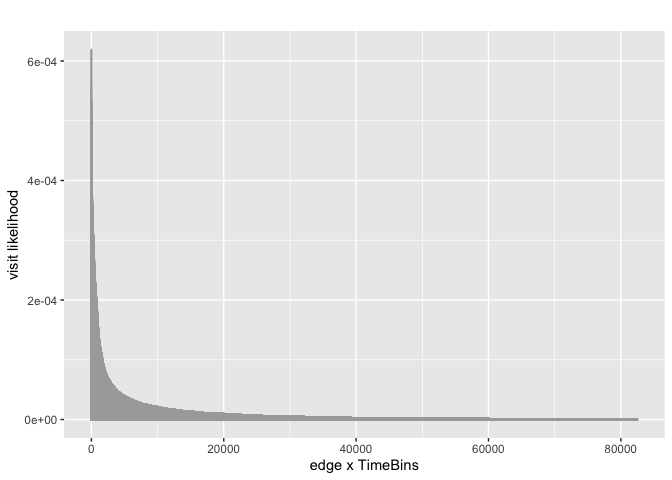
\includegraphics[width=0.45\textwidth]{img/visit_likelihood.png}
    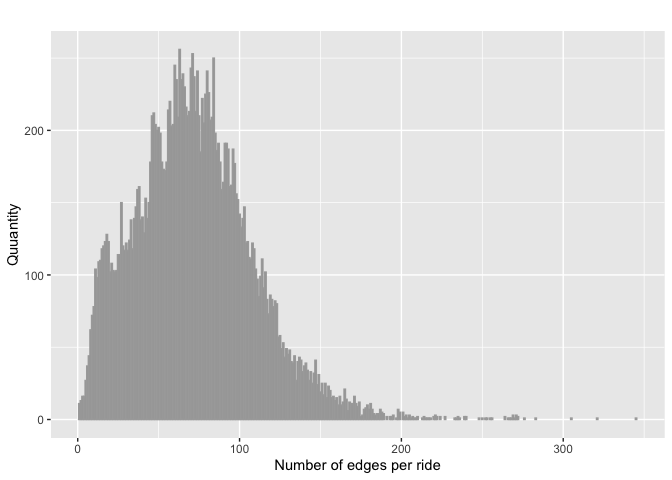
\includegraphics[width=0.45\textwidth]{img/edges_per_ride.png}\\[4pt]
    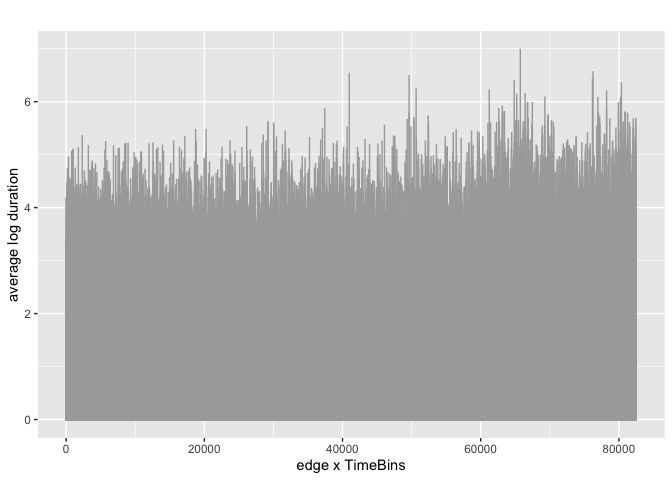
\includegraphics[width=0.45\textwidth]{img/edge_mean_logdur.png}
    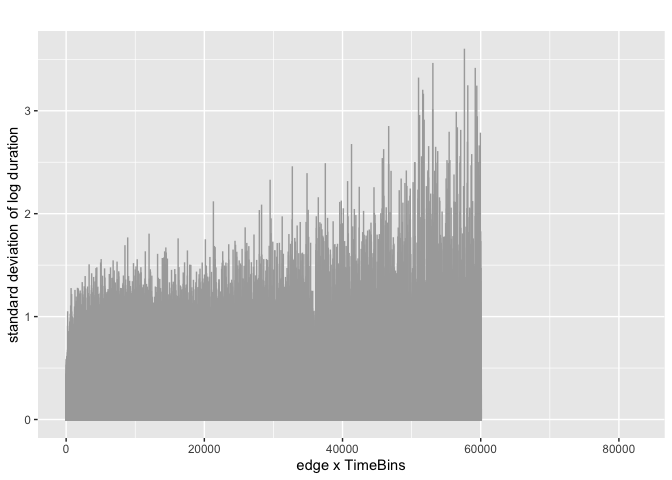
\includegraphics[width=0.45\textwidth]{img/edge_sd_logdur.png}
    \caption{Descriptive statistics of the edge $\times$ time-bin representation in QCD.
    (Top left) Empirical visit likelihood of edge $\times$ time-bin states, sorted in
    decreasing order: a small fraction of states accounts for most observed traffic,
    motivating the frequency-weighted edge sampling in~\eqref{eq:route_sampling}.
    (Top right) Distribution of the number of edges per trip, supporting the
    route-length randomization $\mathrm{Normal}[n,\tau]$ in~\eqref{eq:route_sampling}
    and the large-$n_\path$ regime of
    Lemmas~\ref{lem:population-distribution}--\ref{lem:route-predictive}.
    (Bottom left) Average log travel time per state, approximately flat across states.
    (Bottom right) Standard deviation of log travel time per state, which grows for
    rarer (higher-index) states with smaller sample sizes.}
    \label{fig:edge-timebin-descriptive}
\end{figure}
 

\section{Data Analysis}
\subsection{Outline}
Next, we look at the profit and loss analysis in three scenarios: (1) on-demand rides (known start time and route), (2) scheduled rides (known start time and destination only), and (3) membership rides (unknown start time and route).  

\subsection{Fidelity of sampling process} \label{sec:fedelity}
To test the fidelity of our proposed sampling method, we compare to the empirical distribution of the out-of-sample 2000 test trips in QCD dataset to our sampled travel times and routes. We use the full-order travel time sampler in~\eqref{eq:travel_time_sampling}, alongside three variants of our sampled travel times are used: (1) an independent variant when setting $\xi = 0$; (2) a first-order variant when $(\Sigma)_{ij} =0$ if $\abr{i-j}>1$, and (3) a second-order variant when $(\Sigma)_{ij} =0$ if $\abr{i-j}>2$. In addition, we compare the empirical distribution to the route-invariance population version in~\eqref{eq:travel_time_sampling-population}, and to the alternative a Hidden Markov chain model (HMM) method proposed in~\cite[Algo. 2]{woodard2017predicting}. The HMM mode is implemented with 2 hidden congestion states. 

For each test trip, we sample 1000 travel times for each of the mentioned sampling methods. Those 1000 samples are averaged to produce a single estimate of the test trip travel time. Only a sigle sample per test trips is sampled form the population variant~\eqref{eq:travel_time_sampling-population}, since this method does not require averaging. 

Figure~\ref{fig:fidelity_traveltime}(left) showcases the empirical cumulative distribution of the sampled travel times alongside the 2000 test trips. For our proposed sampling methods, we set $\xi = 0.31$ as shown in~\cite[Tab.~1]{elmasri2020predictive}. High fidelity is observed for all our sampling methods. The fidelity is higher for higher order correlation structures. The full-order sampling method achieves highest fidelity, with the second-order and first-order follow accordingly. Since the population version does not account for series dependency among edges of the trip, it achieves relatively lower fidelity. However, all our sampling method suggest a significant improvement compared to the HMM alternative. 
\begin{figure}[h!tbp]
    \centering
    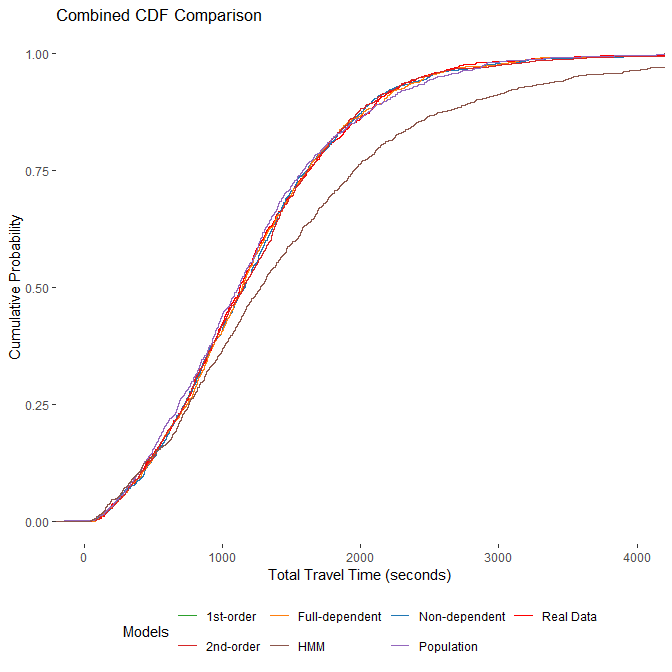
\includegraphics[width=0.45\linewidth]{img/sampled travel times.png}
    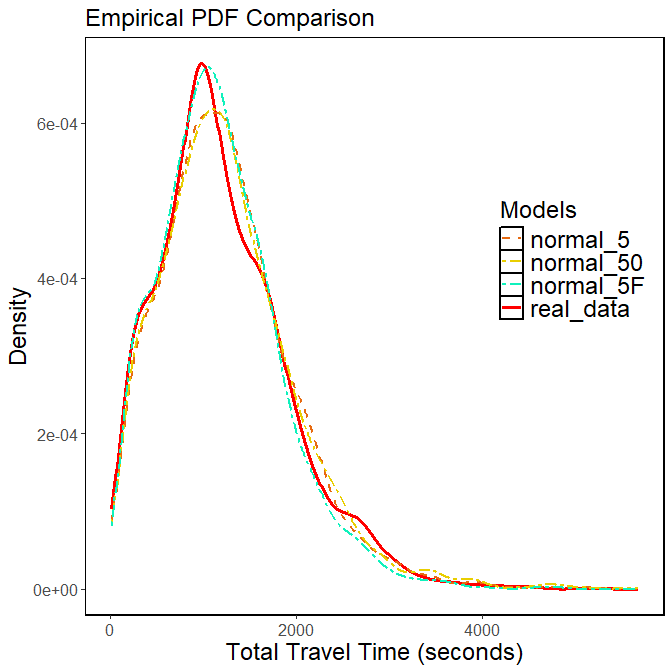
\includegraphics[width=0.45\linewidth]{img/route_sampling_fidelity.png}
    \caption{(Left) Comparing the empirical cumulative distribution of the 2000 test trips, our proposed travel time sampling methods, and the HMM model of~\cite[Algo.~2]{woodard2017predicting}. (Right) Route-varied travel time simulation via~\eqref{eq:route_sampling} under normal and $t$-based edge matching at significance levels $0.05$, $0.50$, and $0.95$.}
    \label{fig:fidelity_traveltime}
\end{figure}

For every travel time sampling method, we additionally vary the observed route of a test trip using~\eqref{eq:route_sampling}. That is, given a trip, we select the set of statistically similar edges $\times$ time bins, following~\eqref{eq:similar-edges}. With this set we sample 5 routes using~\eqref{eq:route_sampling}, and for each sampled route we sample, and average, 1000 travel times from~\eqref{eq:travel_time_sampling}. The travel times for those routes are then averaged to produce a single travel time estimate for the given test trip. The population version~\eqref{eq:travel_time_sampling-population} is route-invariant, as it only dependent on distance, i.e.~the sampled $n'$. The HMM method is omitted here since it does not provide a way to sample routes. 


Figure~\ref{fig:fidelity_traveltime}(right) showcases the empirical cumulative distribution of the sampled travel times alongside the 2000 test trips when routes are resampled via~\eqref{eq:route_sampling} with $\tau = 0$ in~\eqref{eq:route_sampling} (i.e.\ no route-length perturbation beyond similar-edge resampling). High fidelity is observed for normal edge matching with $F$-test standard-deviation selection at the $5\%$ significance level; similarly, the $t$-based and frequency-weighted variants track the empirical curve closely, while loosening the similarity threshold degrades fidelity.


\begin{figure}[h!tbp]
    \centering
    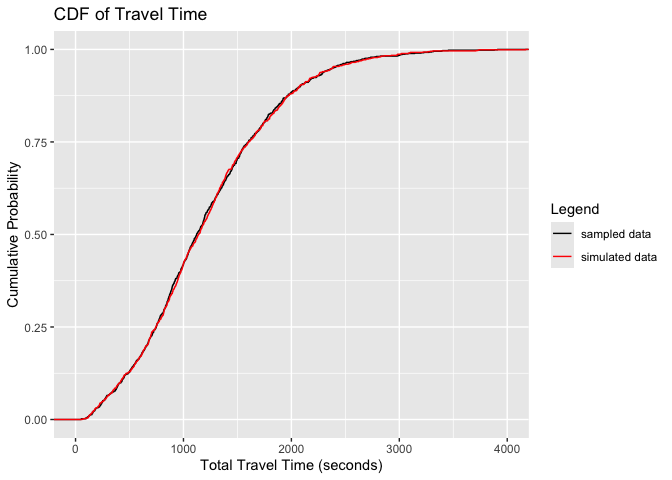
\includegraphics[width=0.6\textwidth]{img/fidelity_fulldep.png}
    \caption{Empirical CDF of realized versus simulated trip travel time using the
    full-order dependent sampler~\eqref{eq:travel_time_sampling} over 1000 QCD trips;
    the two distributions are nearly indistinguishable.}
    \label{fig:fidelity-fulldep}
\end{figure}

\subsection{Profit and loss calculation}
We mimic real-world scenarios\footnote{Extracted from Uber Inc pricing webpage for Quebec City, Canada.} for profit and loss analysis by setting $C_0 = 3.17$CAD, $C_1=0.31$CAD/min and $C_2=0.9$CAD/km for in~\eqref{eq:european-knock-in} for QCD. We calculate the profit as 
\[
\textsf{Total Profit} = \underbrace{R(t,t_0, \rho, K) }_\textsf{Premium} + \underbrace{ K}_\textsf{upfront price} -\underbrace{P_\path(s_1,t_1)}_\textsf{Realized price}.
\]

\[
\textsf{Marginal profit} = {R(t,t_0, \rho, K) } - \max\cbr{{P_\path(s_1,t_1)} - K,0}\one_{\cbr{P_\path(\pend, t_1) \geq Ke^\zeta}}. 
\]

Our analysis sets $K$ to be an estimate of the expected price at start time $t_0$, that is $ K = \hat \EE\sbr{P_\path\rbr{\pstart, t_0}}$, unless otherwise specified. We provide to estimates for $\EE\sbr{\T_\path}$ and $\Var\sbr{\T_\path}$, that are used in the price and premium calculation. The first integrates route information (trip-specific, Lemma~\ref{lem:route-predictive}) and the second is route-invariant (population) version, Lemma~\ref{lem:population-distribution}. The next section presents the parameter estimation for those models. 


\subsection{Traffic parameter estimation}
The population version requires the estimation of only two parameters $\cbr{\mu, \sigma}$.~\cite{elmasri2020predictive} used the sample mean $\hatmu$ is an unbiased estimator for $\mu$, and provided a profile estimator $\sigmaprofile$ for $\sigma^2$ in. We calculate those estimators from 1,000 trips sampled at-random from the training data according to each stratum (rush, Non-rush). Refer to~\citet[Sec.~3.3.2]{elmasri2020predictive} for detailed description of the estimation method. We found that sampling more than 1,000 trips did not lead to significantly different estimates than those in Table~\ref{tb:parameter-estimates}.
\begin{table}[!htp]
  \centering
    \caption{Parameter estimation under different sampling methods}
    \label{tb:parameter-estimates}
    {\footnotesize 
  \begin{tabular}{l lllll}
    %\toprule
                      & \multicolumn{3}{c}{Sampling method}                                \\
     %                  \cmidrule{2-4}
                      & At random         & \multicolumn{2}{c}{Stratified by traffic-bins} \\[5pt]
                     
    %\cmidrule{2-4}
                      &                   & {rush} & {Non-rush}                         \\
   % \midrule                                                 
    \(\hatmu\)        & 16.46             & 17.34     & 13.70                              \\   
    \(\sigmaprofile\) & 25.18             & 26.91     & 18.44                              \\
    \midrule
    \(\hatxi\)        & 0.30              & 0.31     & 0.29                               \\
    \(\hatnu\)        & 1.74              & 2.04      & 1.15
%    \bottomrule
  \end{tabular}
  }
\end{table}

The trip-specific version requires the integration of route information by estimating the edge-specific sample mean and variance pair \(\{\hatm_{e}, \hatsigma_{e}\}\) for each traffic-bin. The whole training data is used to estimate those parameters. 

Following the methodology of \cite{elmasri2020predictive}, we estimate the correlation parameter $(\xi)$ and residual variance $(\nu)$ defined in Lemma~\ref{lem:route-predictive}. We generated estimates $(\hatxi, \hatnu)$ under two conditions: first, for stratified rush and Non-rush periods using 4,000 trips from each, and second, for a non-stratified baseline using 4,000 trips from the entire training data. The results are presented in Table~\ref{tb:parameter-estimates}. $\hatxi$ is a profile estimator of $\xi$, see~\citet[Sec.~3.4]{elmasri2020predictive} for more details. All resulting estimates are reported in Table~\ref{tb:parameter-estimates}.

Compared to non-rush periods, rush hour travel is slower (17.3s vs 13.7s average) and significantly more unpredictable. This is reflected in a higher standard deviation (26.91 vs 18.44) and similar correlation.

\subsection{Sensitivity analysis to the strike price $K$}\label{sec:Sensitivity analysis to the strike price}
Rideshare markets promise an upfront price $K$ as an estimate of the expected price $P_{\rbr{\pstart, \pend}}(\pstart, t_0)$ at start (location, time) = $(\pend, t_0)$, as the exact expectations is unknown. Complex machine learning methods are responsible in producing this estimate which is shown to the consumer. To assess method variability to strike price choice, we study two scenarios:~\ref{on-demand} on-demand rides (known route and start time) and~\ref{scheduled} scheduled rides (known start time and destination). For both cases, we will set the risk-free rate $r=0$, and vary the minimum cutoff threshold $\zeta \in \cbr{0, 0.1}$. The solution to \eqref{eq:european-knock-in} simplifies to 
\begin{equation}\label{eq:price-when-r=0}
R(t_0,t_0, \rho, K) = (d_0-K)\cbr{1- \Phi(d_1)} + C_1d_1\phi(d_1),
\end{equation} 
where 
\[
d_0 = C_0 + C_1\EE[\T_\path] + C_2\delta_\path, \qquad
d_1 = \frac{Ke^\zeta -d_0}{C_1\cbr{\Var[\T_\path]}^{1/2}}.
\]
We will assume that the strike price $K$ is the most accurate prediction of the expected price at start time $t_0$, as set it to $K = \hat P_\path(\pstart, t_0)e^{i}$, for $i \in \cbr{0, 0.1}$, where $\hat P_\path(\pstart, t_0)$. In the case that $i= 0$ this will set $d_0 - K=0$ in~\eqref{eq:price-when-r=0}. 
    
We estimate the expected value $\EE[\T_\path]$ and $\Var[\T_\path]$ using the developed travel time and route sampling methods in Section~\ref{sec:sampler}, for the trip-specific and population versions. For each test trip, we sample 1000 travel times for each of our sampling methods. Those 1000 samples are averaged to produce a single estimate of the test trip expected travel time. The sample variance of those sample is an estimate of $\Var[\T_\path]$. Only a single sample per test trips is sampled form the population variant~\eqref{eq:travel_time_sampling-population}, since this method does not require averaging. Those values are then inputted in~\eqref{eq:price-when-r=0}, alongside the strike price, to estimate the price guarantee premium. 

Figure~\ref{fig:route-specific-R} illustrates the pricing guarantee premium ($R(t_0,t_1,t_0, 4, A)$) for the 2000 test trips against estimated time and true distance, when the premium is computed for the trip-specific and population version, setting $K= P_\path(\pstart, t) $, and $\zeta = 0$. The trip-specific premium is twice smaller than the population versions (right panel), with premium increasing linearly by distance or travel time. All premiums are less than 2CAD, except for one trip. This suggest an empirical upper bound guaranteeing pricing in rideshare. For example, around 4 KM, the average price for the trip guarantee is 0.21\$, with maximum at 0.49\$ and minimum at 0.03\$. For example, 52cents is all it takes to guarantee a price of a 4~KM arbitrary ride at $K=3.17+0.31 \times0.0982\times4000/60+0.9\times 4 = 8.8$CAD. Knowing the actual route leads to cheaper pricing of of this guarantee.
\begin{figure}
    \centering
    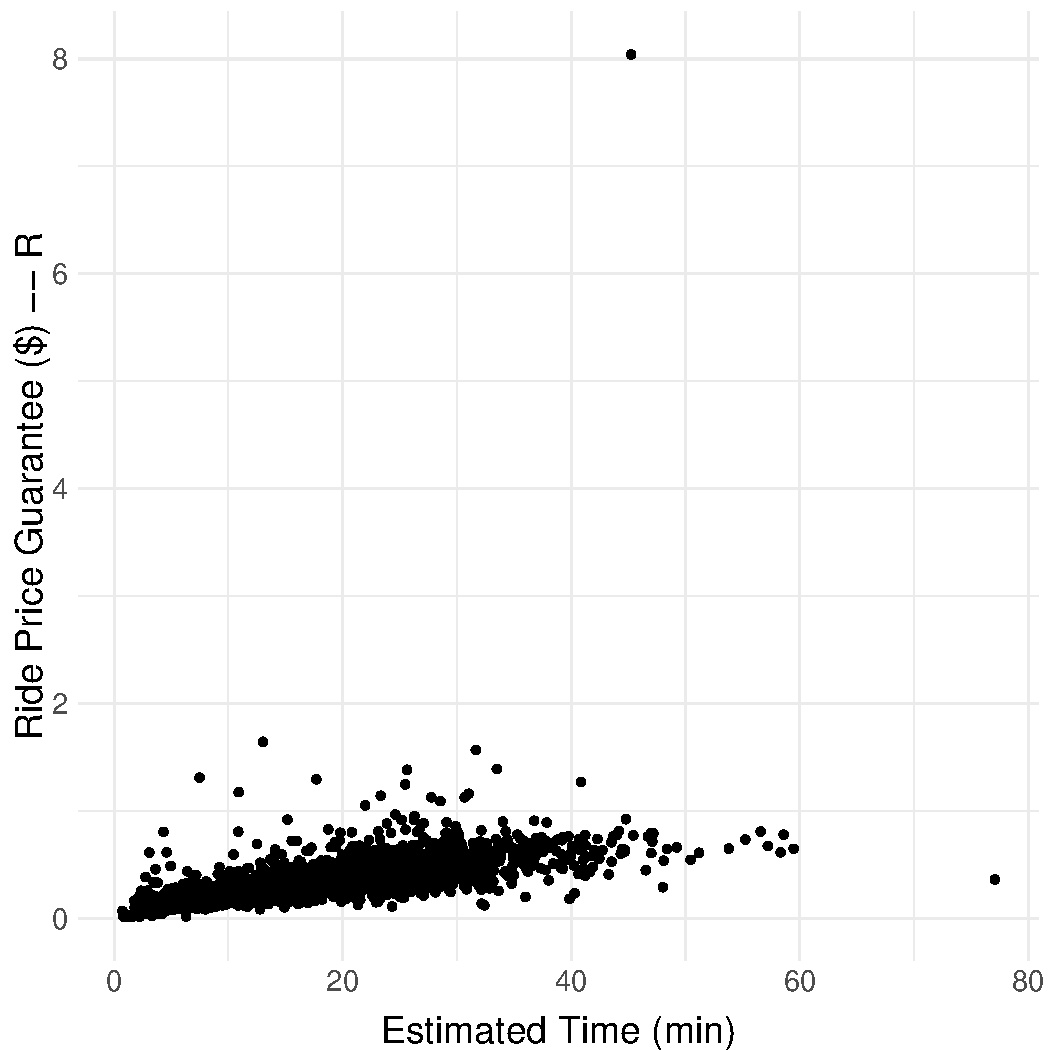
\includegraphics[width=0.32\textwidth]{img/R-example.pdf}
    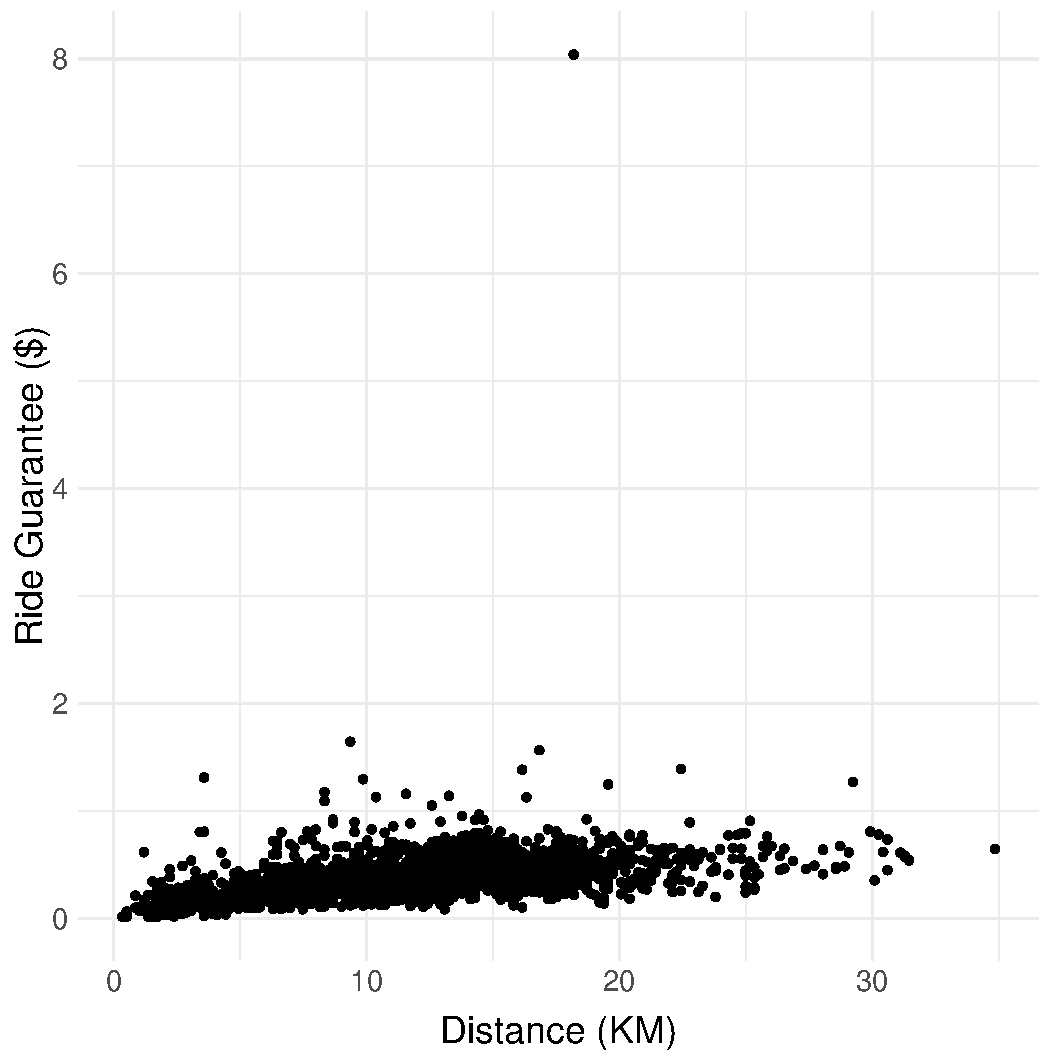
\includegraphics[width=0.32\textwidth]{img/R-example-distance.pdf}
    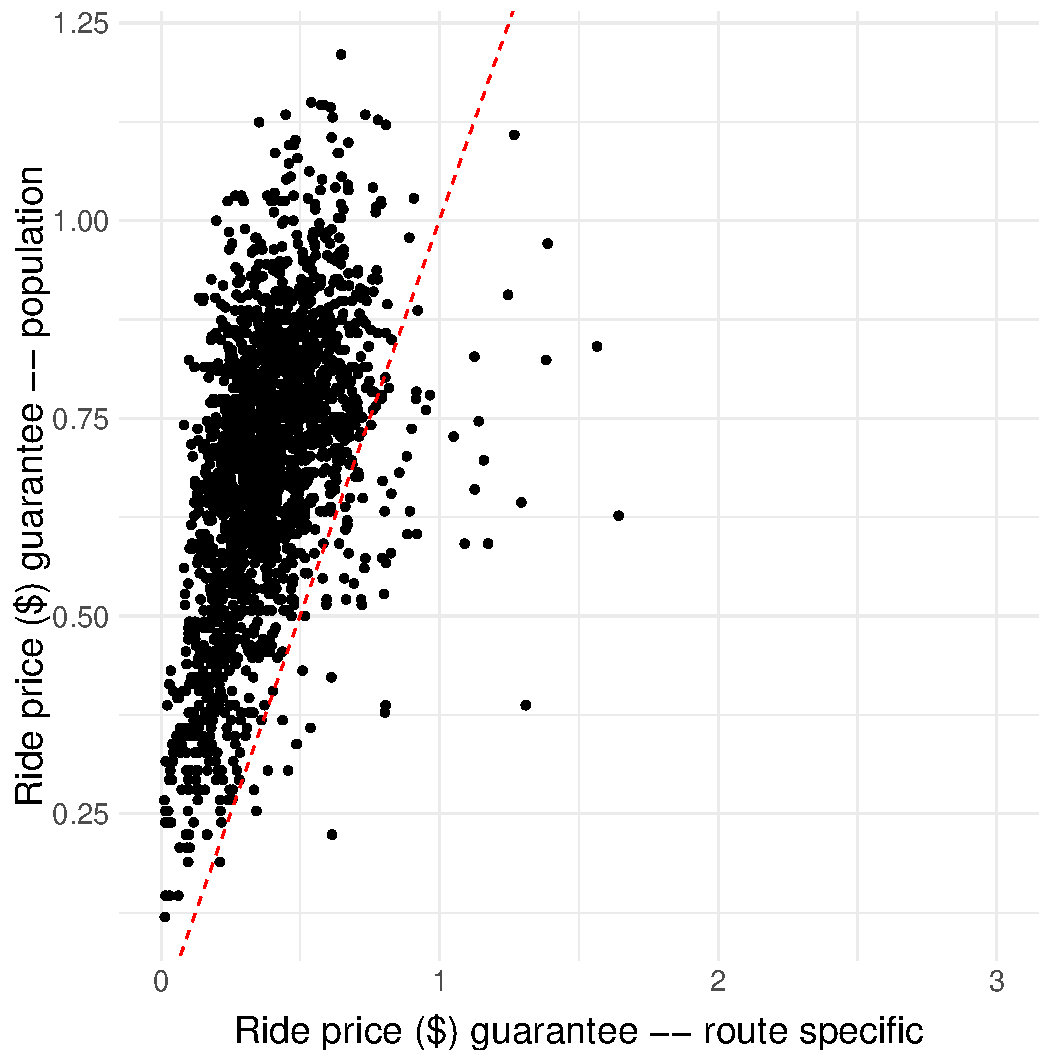
\includegraphics[width=0.32\textwidth]{img/R_route_vs_pop.pdf}
    \caption{Premiums of on-demand~\ref{on-demand} scenario for 2000 test trips in QCD, while setting $K=P_\path(\pstart, t_0)$, as the expected price at the start (location, time) $=(\pstart, t_0)$.}
    \label{fig:route-specific-R}
\end{figure}

Figure~\ref{fig:profit_loss} (right) show the theoretical profit breakdown of our pricing method. Where Maximum profit is achieved is the actual price is less than the strike price $K$. This profit decreases gradually until the breakeven point $R + K$. The loss increases afterwards, with a limited cap, since rides in real-world networks have limited time. The Left panel shows show the profit and loss per trip for each of the sampled method {\color{red} (plot y-axis profit/loss range from negative to positive, x-axis distance, profit is computed as is~\eqref{eq:ride-cost}.}


\begin{figure}[h!]
\centering
\includegraphics[width=0.32\textwidth]{img/average_trips_per_weekhour.pdf}
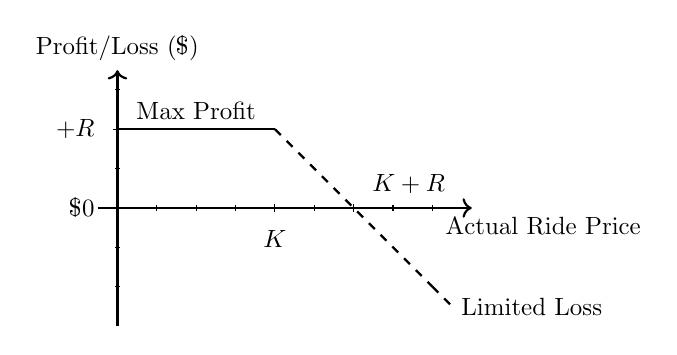
\begin{tikzpicture}[scale=0.5, every node/.style={scale=0.9}]
    % Define coordinates
    \coordinate (Origin) at (0,0);
    \coordinate (K) at (4,0);
    \coordinate (R_val) at (0,2);
    \coordinate (KR) at (6,0);
    \coordinate (TurnPoint) at (4,2);
    \coordinate (LowP) at (0,2);
    \coordinate (HighP_End) at (8,-2);
    \coordinate (HighP_Ext) at (8.5,-2.5);

    % Draw axes
    \draw[->, thick] (-0.5,0) -- (9,0) node[below right, xshift=-5mm] {Actual Ride Price};
    \draw[->, thick] (0,-3) -- (0,3.5) node[above] {Profit/Loss (\$)};

    % Draw tick marks on X-axis
    \draw (4,3pt) -- (4,-3pt) node[below=4pt] {$K$};
    \draw (6,3pt) -- (6,-3pt) node[above right=4pt] {$K+R$};
    \foreach \x in {1,2,3,5,7,8} \draw (\x,2pt) -- (\x,-2pt);

    % Draw tick marks on Y-axis
    \draw (3pt,2) -- (-3pt,2) node[left=4pt] {$+R$};
    \draw (3pt,0) -- (-3pt,0) node[left=4pt] {\$0};
    \foreach \y in {-2,-1,1,3} \draw (2pt,\y) -- (-2pt,\y);

    % Draw the profit/loss lines
    \draw[thick] (LowP) -- (TurnPoint) node[midway, above] {Max Profit};
    \draw[thick, dashed] (TurnPoint) -- (HighP_End);
    \draw[thick, dashed] (HighP_End) -- (HighP_Ext) node[right] {Limited Loss};
\end{tikzpicture}
\caption{(Left placeholder) Estimated profit and loss of 2000 test trips. (Right) Theoretical profit and loss analysis.}
\label{fig:profit_loss}
\end{figure}

Table~\ref{tab:strike-metrics} reports guarantee performance across strike prices.
As the strike rises from the expected price ($\times 1$) to a 10\% markup
($\times e^{0.1}$), the guarantee triggers less often and the share of profitable
trips increases from 0.75 to 0.92 for the population model and from 0.67 to 0.95 for
the trip-specific model, while the average premium falls correspondingly. The premium
is modest throughout, between 0.4\% and 4.4\% of the trip price. Consistent with
Figure~\ref{fig:route-specific-R}, the trip-specific premium is roughly half the
population premium at every strike (for example, 2.15\% versus 4.43\% at $\times 1$),
reflecting the tighter variance obtained by conditioning on the route. Both models
remain profitable on average (profit factor $>1$), but the population model carries a
larger downside, with a worst-case single-trip loss near \$$29$ against \$$22$ for the
trip-specific model.
\begin{table}[h!]
    \centering
    \caption{On-demand price-guarantee performance under different strike prices,
    with $r=0$ and $\zeta=0$, over 10{,}000 trips. Profit and premium in CAD;
    profit factor is the ratio of total gains to total losses.}
    \begin{tabular}{l l c c c c c}
    \hline
    Model & Strike & \% profitable & Avg.\ profit & Max.\ loss & Profit factor & Premium/$P$ (\%) \\
    \hline
    Population    & $\times 1$        & 0.75 & 0.18 & $-28.79$ & 1.39 & 4.43 \\
                  & $\times e^{0.05}$ & 0.84 & 0.11 & $-27.58$ & 1.41 & 2.35 \\
                  & $\times e^{0.1}$  & 0.92 & 0.04 & $-25.88$ & 1.36 & 1.11 \\
    Trip-specific & $\times 1$        & 0.67 & 0.04 & $-21.85$ & 1.12 & 2.15 \\
                  & $\times e^{0.05}$ & 0.87 & 0.03 & $-20.73$ & 1.23 & 0.73 \\
                  & $\times e^{0.1}$  & 0.95 & 0.05 & $-19.36$ & 1.99 & 0.36 \\
    \hline
    \end{tabular}
    \label{tab:strike-metrics}
\end{table}

\subsection{Discount memberships}
Consider the case of a monthly membership~\ref{membership} with a 10\% discount on-demand rides. Setting $K = P_\path(\pstart,t_1)e^{-\zeta}$ in~\eqref{eq:ride-cost}, where $P_\path(\pstart t_1)$ is the expected price at (start time, location) = $(t_1, \pstart)$, with cutoff threshold at $\zeta = \cbr{0,0.1}$. 

With the 2000 test trips of QCD, we uniformly sample $M=40$ from the first month and dedicate them as a counterfactual rider. For every pair of (start time, route)$=(t_k, \path_k)$, $k = 1, \dots, 40$, we compute the actual $P_{\path_k}(\pend)$ prices. No ride information are known at the membership subscription time. Therefore, we estimate the membership cost, as the sum of premiums of potential rides, we mimic the distribution of potential rides as follows. For each day $y=1, \dots, 30$, we sample the number of potential rides $M_y$, the time of bin of the rides and taken route $(b_k, \path_k), k=1, \dots, M_y$
\begin{equation} \label{eq:counterfactual_rider}
\begin{aligned}
    M_y & \sim \textsf{Binomial} (2, 2/3) \\
    b_k & \sim \textsf{Uniform}\sbr{\textsf{AM-rush, PM-rush, Otherwise}}, \quad k = 1, \dots, M_y \\
    \path_k & \sim \textsf{Uniform over rides in } {b_k} \textsf{ in the train set} \\
\end{aligned}
\end{equation}

We set the Binomial probability to $2/3$, such that $30 \times 2 \times p = 40$. This sampling process can be adjusted accordingly given a rider history. Sampling $M_y$ is not required if the membership is fixed to $M$ rides. 

For every route in~\eqref{eq:counterfactual_rider}, we sample 100 starting times $\T_{\path_k}$ using~\eqref{eq:travel_time_sampling}, and estimate the route premiums. For each day, we repeat this process 10 times, and average all the premiums as the average premium per day. The membership cost is the sum of all the average premiums over 30 days. 

Figure~\ref{fig:profit_loss_discount} showcases the profit and loss analysis of such a membership structure with respect to distance (left panel) and the number of days in the month the ride has been taken (right panel)

\begin{figure}[h!]
\centering
\includegraphics[width=0.32\textwidth]{img/average_trips_per_weekhour.pdf}
\includegraphics[width=0.32\textwidth]{img/average_trips_per_weekhour.pdf}
\caption{(Left placeholder) Estimated profit and loss of 2000 test trips. (Right) Theoretical profit and loss analysis.}
\label{fig:profit_loss_discount}
\end{figure}

Table~\ref{tab:discount-metrics} shows the effect of bundling a 10\% discount
($K = 0.9\,P$) into the membership. The discount reverses the ranking observed in the
on-demand case: the population model remains slightly profitable, with an average
return of $2.7$--$2.9\%$, whereas the thinner trip-specific premium no longer covers
the discounted guarantee and turns marginally loss-making, with an average return of
$-0.4$ to $-0.5\%$. Introducing a non-zero cutoff $\zeta = 0.1$ lowers the premium
charged to the rider but also erodes the provider's margin and deepens the worst-case
loss, since fewer overruns are recovered.
\begin{table}[h!]
    \centering
    \caption{Discount-membership performance with $K = 0.9\,P$ under different cutoff
    thresholds $\zeta$, over 100 trips. Profit and premium in CAD; return in \%.}
    \begin{tabular}{l l c c c c}
    \hline
    Model & Cutoff $\zeta$ & Avg.\ \% return & Avg.\ profit & Max.\ loss & Premium/$P$ (\%) \\
    \hline
    Population    & $0$   & $2.86$  & $0.09$  & $-8.41$ & 11.42 \\
                  & $0.1$ & $2.71$  & $-0.03$ & $-9.28$ &  9.73 \\
    Trip-specific & $0$   & $-0.45$ & $-0.23$ & $-6.90$ & 10.49 \\
                  & $0.1$ & $-0.53$ & $-0.36$ & $-7.99$ &  7.90 \\
    \hline
    \end{tabular}
    \label{tab:discount-metrics}
\end{table}
\subsection{Membership Abuse}
\label{membership_abuse}
Ridership behaviour can change under discounted prices, for example, a rider might start taking longer routes than anticipated, or more routes at the rush hours (having higher prices). We sample a 100 different counterfactual rider of 40 riders each, uniformly with replacement from the test trips. For each rider, we set $M_1 \leq 40$ trips to be from the upper $q$ quantile of the longest trips in the data. For example $M_1 = 10$, and $q=0.9$ would sample (with replacement) 10 rides (out of 40) from the highest 10\% of rides in the test trip.
\begin{table}[ht]
\centering
\caption{\textbf{\% Average Return at Different Pressure Settings}}
\begin{tabular}{l | *{9}{r}}
\toprule
\multicolumn{1}{c|}{\footnotesize{$M_1/40$}} & \multicolumn{9}{c}{$q$} \\ 
 \cmidrule(lr){2-10} 
 {\footnotesize }& 0.1    & 0.2     & 0.3      & 0.4      & 0.5      & 0.6       & 0.7       & 0.8       & 0.9       \\
\midrule
0    & 4.76 & 6.06 & 5.24 & 3.98 & 3.87 & 3.09 & 3.60 & 3.26 & 4.09 \\
0.1  & 5.04 & 3.56 & 2.26 & 0.80 & 0.63 & 0.32 & 0.53 & -0.52 & 0.82 \\
0.2  & 4.71 & 3.39 & -0.91 & -0.39 & -2.10 & -4.01 & -6.47 & -7.55 & -8.57 \\
0.3  & 2.84 & -5.16 & -1.39 & -2.91 & -4.50 & -8.44 & -9.31 & -12.76 & -13.75 \\
0.4  & 2.18 & -0.08 & -2.96 & -5.94 & -8.90 & -11.92 & -14.56 & -16.06 & -19.84 \\
0.5  & 1.65 & -1.56 & -5.21 & -9.86 & -12.16 & -16.67 & -19.78 & -22.57 & -25.15 \\
\bottomrule
\end{tabular}
\end{table}


\begin{table}[ht]
\centering
\caption{\textbf{\% Standard deviation of Average Return at Different Pressure Settings}}
\begin{tabular}{l | *{9}{r}}
\toprule
\multicolumn{1}{c|}{\footnotesize{$M_1/40$}} & \multicolumn{9}{c}{$q$} \\ 
 \cmidrule(lr){2-10} 
 {\footnotesize }& 0.1    & 0.2     & 0.3      & 0.4      & 0.5      & 0.6       & 0.7       & 0.8       & 0.9       \\
\midrule
0 & 1.38 & 1.32 & 1.35 & 1.35 & 1.35 & 1.38 & 1.33 & 1.37 & 1.39 \\
0.1 & 1.31 & 1.35 & 1.34 & 1.31 & 1.33 & 1.27 & 1.25 & 1.25 & 1.27 \\
0.2 & 1.32 & 1.30 & 1.58 & 1.29 & 1.29 & 1.31 & 1.29 & 1.30 & 1.26 \\
0.3 & 1.35 & 6.28 & 1.44 & 1.33 & 1.26 & 1.34 & 1.30 & 1.29 & 1.27 \\
0.4 & 1.35 & 1.35 & 1.34 & 1.33 & 1.31 & 1.35 & 1.28 & 1.18 & 1.23 \\
0.5 & 1.38 & 1.37 & 1.39 & 1.72 & 1.27 & 1.31 & 1.29 & 1.25 & 1.17 \\
\bottomrule

\end{tabular}
\end{table}

\begin{figure}
    \centering
    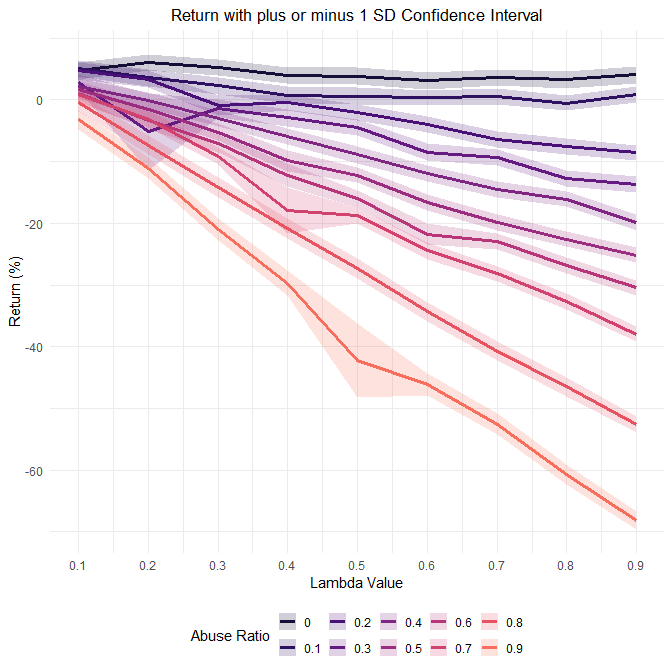
\includegraphics[width=1\linewidth]{sensitive_test.png}
    \caption{Sensitive test result}
    \label{sensitive_test}
\end{figure}
\subsection{Commuter memberships}
Consider the case of 30 commuter ride membership package~\ref{membership}. Fixed at a specific hour of day for a whole month. The start and end locations are fixed and known. Let $K$ be the promised maximum price. 

Here we construct a counterfactual rider by sample uniformly a single trip from the 2000 test trips. Consequently, we randomize it route 29 times and for each route we sample a travel time. This constitute 30 commuter trips, each with a slightly a different route an travel time. We repeat this process 100 times, without replacement, resulting to 100 different counterfactual riders.

For each counterfactual rider we compute the realized price of all 30 commuter trips
and the membership premium $\memebership(t, 30)$ from~\eqref{eq:membership-price},
holding origin--destination fixed and averaging over the 29 randomized routes and
their sampled travel times. The per-rider profit is the collected membership price
minus the sum of realized trip costs. Repeating over the 100 counterfactual riders
yields the distribution of provider profit reported in Table~[X], separately for the
trip-specific and population models. Because the route and start hour are fixed and
only mild route randomization is applied, the premium is substantially tighter than in
the discount-membership case.
% TODO: insert the commuter-membership numbers/table once that run is available.


\section{Discussion} \label{sec:discussion}
In turn, providers build complex models that attempt a sweet spot between profitability and competitiveness. Such predictive models often rely on point-estimates of travel time without accounting for travel uncertainty. Integrating of uncertainty in pricing structures proved elusive for two reasons; (a) analytical approaches are still lacking, and
\bibliographystyle{plainnat}
\bibliography{references}


\begin{appendices}
    


\section{On Demand Simulation}\label{sec:on demand simulation}
This simulation is developed based on \citet{melmasri_traveltimeCLT_sample_ride}. Use the time of drivers entering an edge, we made five different time bins, EveningRush, weekday, MorningRush, EveningNight, and weekendday.  The time bins are set by the R functions in the traveltimeCLT package related to the paper \cite{elmasri2020predictive}. The time difference of the driver entering the first and the next edge is the duration to pass the edge. We then calculate the mean and the standard deviation of the log duration that passes the edge in these time bins. This produced our edge $\times$ time bin dataset. 

Then we randomly sampled $1000$ trips, knowing the route, speed, and time bin, the task is to predict the duration of the entire trip. For every step $e$, we use the mean and sd in the edge $\times$ time bin dataset with the same time bin and the edge ID(denote them as $m_e(t)$ and $\sigma_e(t)$) to predict the duration $\T_e$:
    $${\T_e}=\exp\left(m_e(t)+\sigma_e(t)\Phi^{-1}(U)\right). $$
Here, $\Phi^{-1}(\cdot)$ is the quantile function of the standard normal distribution, and $U$ is some uniform distribution that ranged from $0$ to $1.$ The simulated entire trip time is then given by $\hat{\T_\rho}=\sum_{e\in\rho}\hat{\T_e}$.

The duration of drivers on different edges of the trip may not be independent. So the uniform distribution in one trip should have some dependent structure. We proposed an independent model and three dependent structures, first-order, second-order, and full-dependent models. The dependency is set to be $0.31$, which is recommended in the \cite{elmasri2020predictive}. The correlation matrix for the dependent model is $\Sigma_t$, calculated by:$$\Sigma_1=\begin{bmatrix}
        1 & 0.31 &0.31^2 & 0.31^3&...  \\
        0.31 & 1 & 0.31 & 0.31^2&...\\
        0.31^2 & 0.31 & 1 & 0.31&...\\
        0.31^3 & 0.31^2 & 0.31 & 1&...\\
        ... & ... & ... & ...&...\\
    \end{bmatrix}, \Sigma_t=[ 2 \times \sin(\sigma \times \pi/6)]_{\forall \sigma\in \Sigma_1}.$$
The transform ensures that $\Sigma_t$ is a positive definite matrix. Following a similar idea, the first-order and second-order correlation matrices are transformed from $\Sigma_2$ and $\Sigma_3$, respectively. $\Sigma_2$ and $\Sigma_3$ are as follow:
$$\Sigma_2=\begin{bmatrix}
        1 & 0.31 &0 & 0&...  \\
        0.31 & 1 & 0.31 & 0&...\\
        0 & 0.31 & 1 & 0.31&...\\
        0 & 0 & 0.31 & 1&...\\
        ... & ... & ... & ...&...\\
        \end{bmatrix},
        \Sigma_3=\begin{bmatrix}
        1 & 0.31 &0.31^2 & 0&...  \\
        0.31 & 1 & 0.31 & 0.31^2&...\\
        0.31^2 & 0.31 & 1 & 0.31&...\\
        0 & 0.31^2 & 0.31 & 1&...\\
        ... & ... & ... & ...&...\\\end{bmatrix}$$
This time, we use the nearPD function in the Matrix package to find the nearest correlation matrix \cite{higham2002computing}. 

We also included the population model in \cite{elmasri2020predictive}, and the HMM model in \cite{woodard2017predicting} for comparison. Plot \ref{simulation_plot1} demonstrated these results. We found that all four models we proposed worked very well. The population model's predictions have more errors but are generally acceptable. The HMM model overestimated the time of all trips. The effect of different dependence structures is not significant. The non-dependent prediction is already very close to perfect so we cannot see improvements.
\begin{figure}[h!tbp]
    \centering
    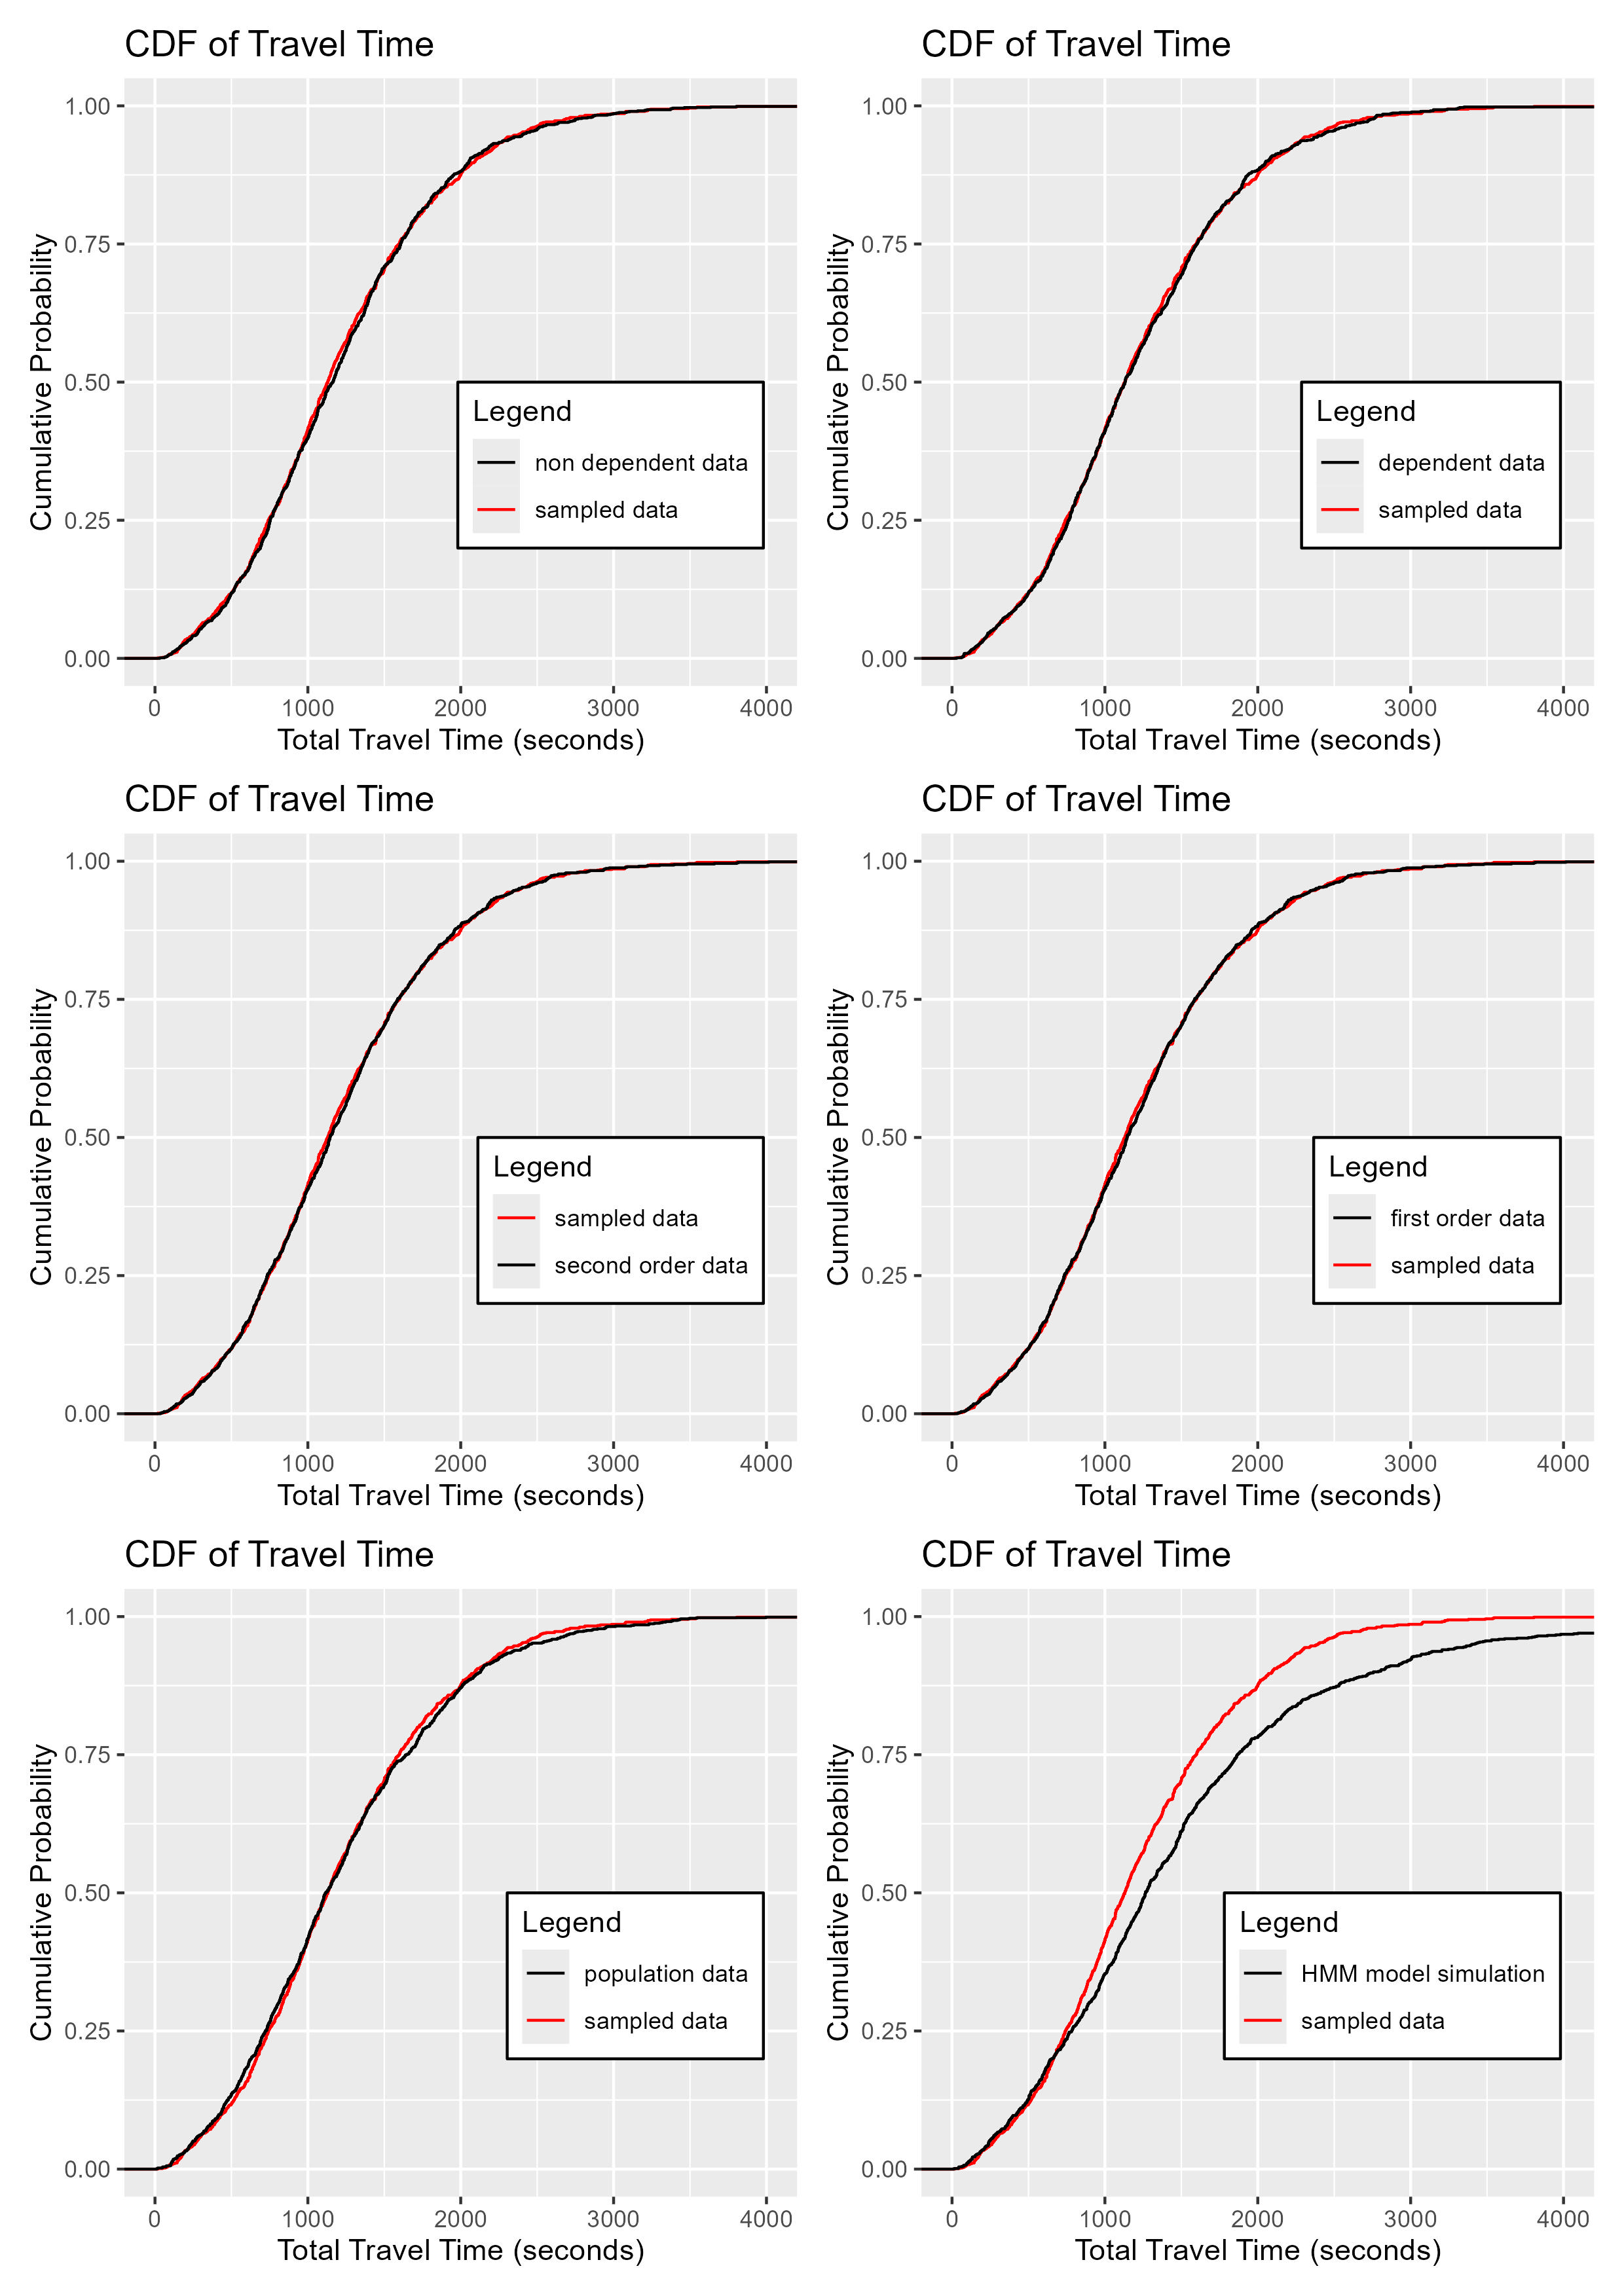
\includegraphics[width=\linewidth]{img/R_combined_simulation_plots.jpg}
    \caption{Simulation results of different models}
    \label{simulation_plot1}
\end{figure}
\section{Construction of the Metric graph}\label{sec:Construction of the Metric graph}
Every trip passes a series of edges. We record the first and next edge numbers from these trips. For instance, given a trip traveled $1,6541,6494$, then we know that we can go from $1$ to $6541$, and $6541$ to $6494$. Later, we observed another trip going $1,6494,6497$, then we knew there were some crossroads, so edge $1$ is connected with $6541$ and $6494$, and drivers can enter edge $6494$ from $1$ and $6541$. We go through all trips in the dataset and record the connections. In addition to the edge $\times$ time bin dataset, we made a new data table that categorizes by connections and time bins. In our example, we will record the statistics of $1$ to $6541$, $6541$ to $6494$, $1$ to $6494$, and $6494$ to $6497$. In the new connection $\times$ time bin dataset, the duration from the beginning of edge $e_1$ to the beginning of edge $e_2$ is denoted by $\T_{e_1,e_2}$, and it follows the formula below:

$${\T_{e_1,e_2}}=\exp\left(m_{e_1,e_2}(t)+\sigma_{e_1,e_2}(t)\Phi^{-1}(U)\right).$$

We randomly selected $20$ trips from the trip dataset. We plot a simplified metric graph based on the sampled $20$ trips. In figure \ref{network_plot1}, green points refer to the starting edge, and red points are the second last edge of the trip. We assume that all drivers begin on the starting point of the starting edge, and stop at the beginning of the last edge. Yellow points refer to the crossroads. In the real data, there may be dozens of edges between crossroads, starting and ending. We simplify these long ``normal" edge series to $6$ arrows. We already see many crossroads in the plot. Given the $23054$ trips in the QCD trip dataset, we will have a super large and complex metric graph with crossroads on almost every trip.
\begin{figure}[h!tbp]
    \centering
    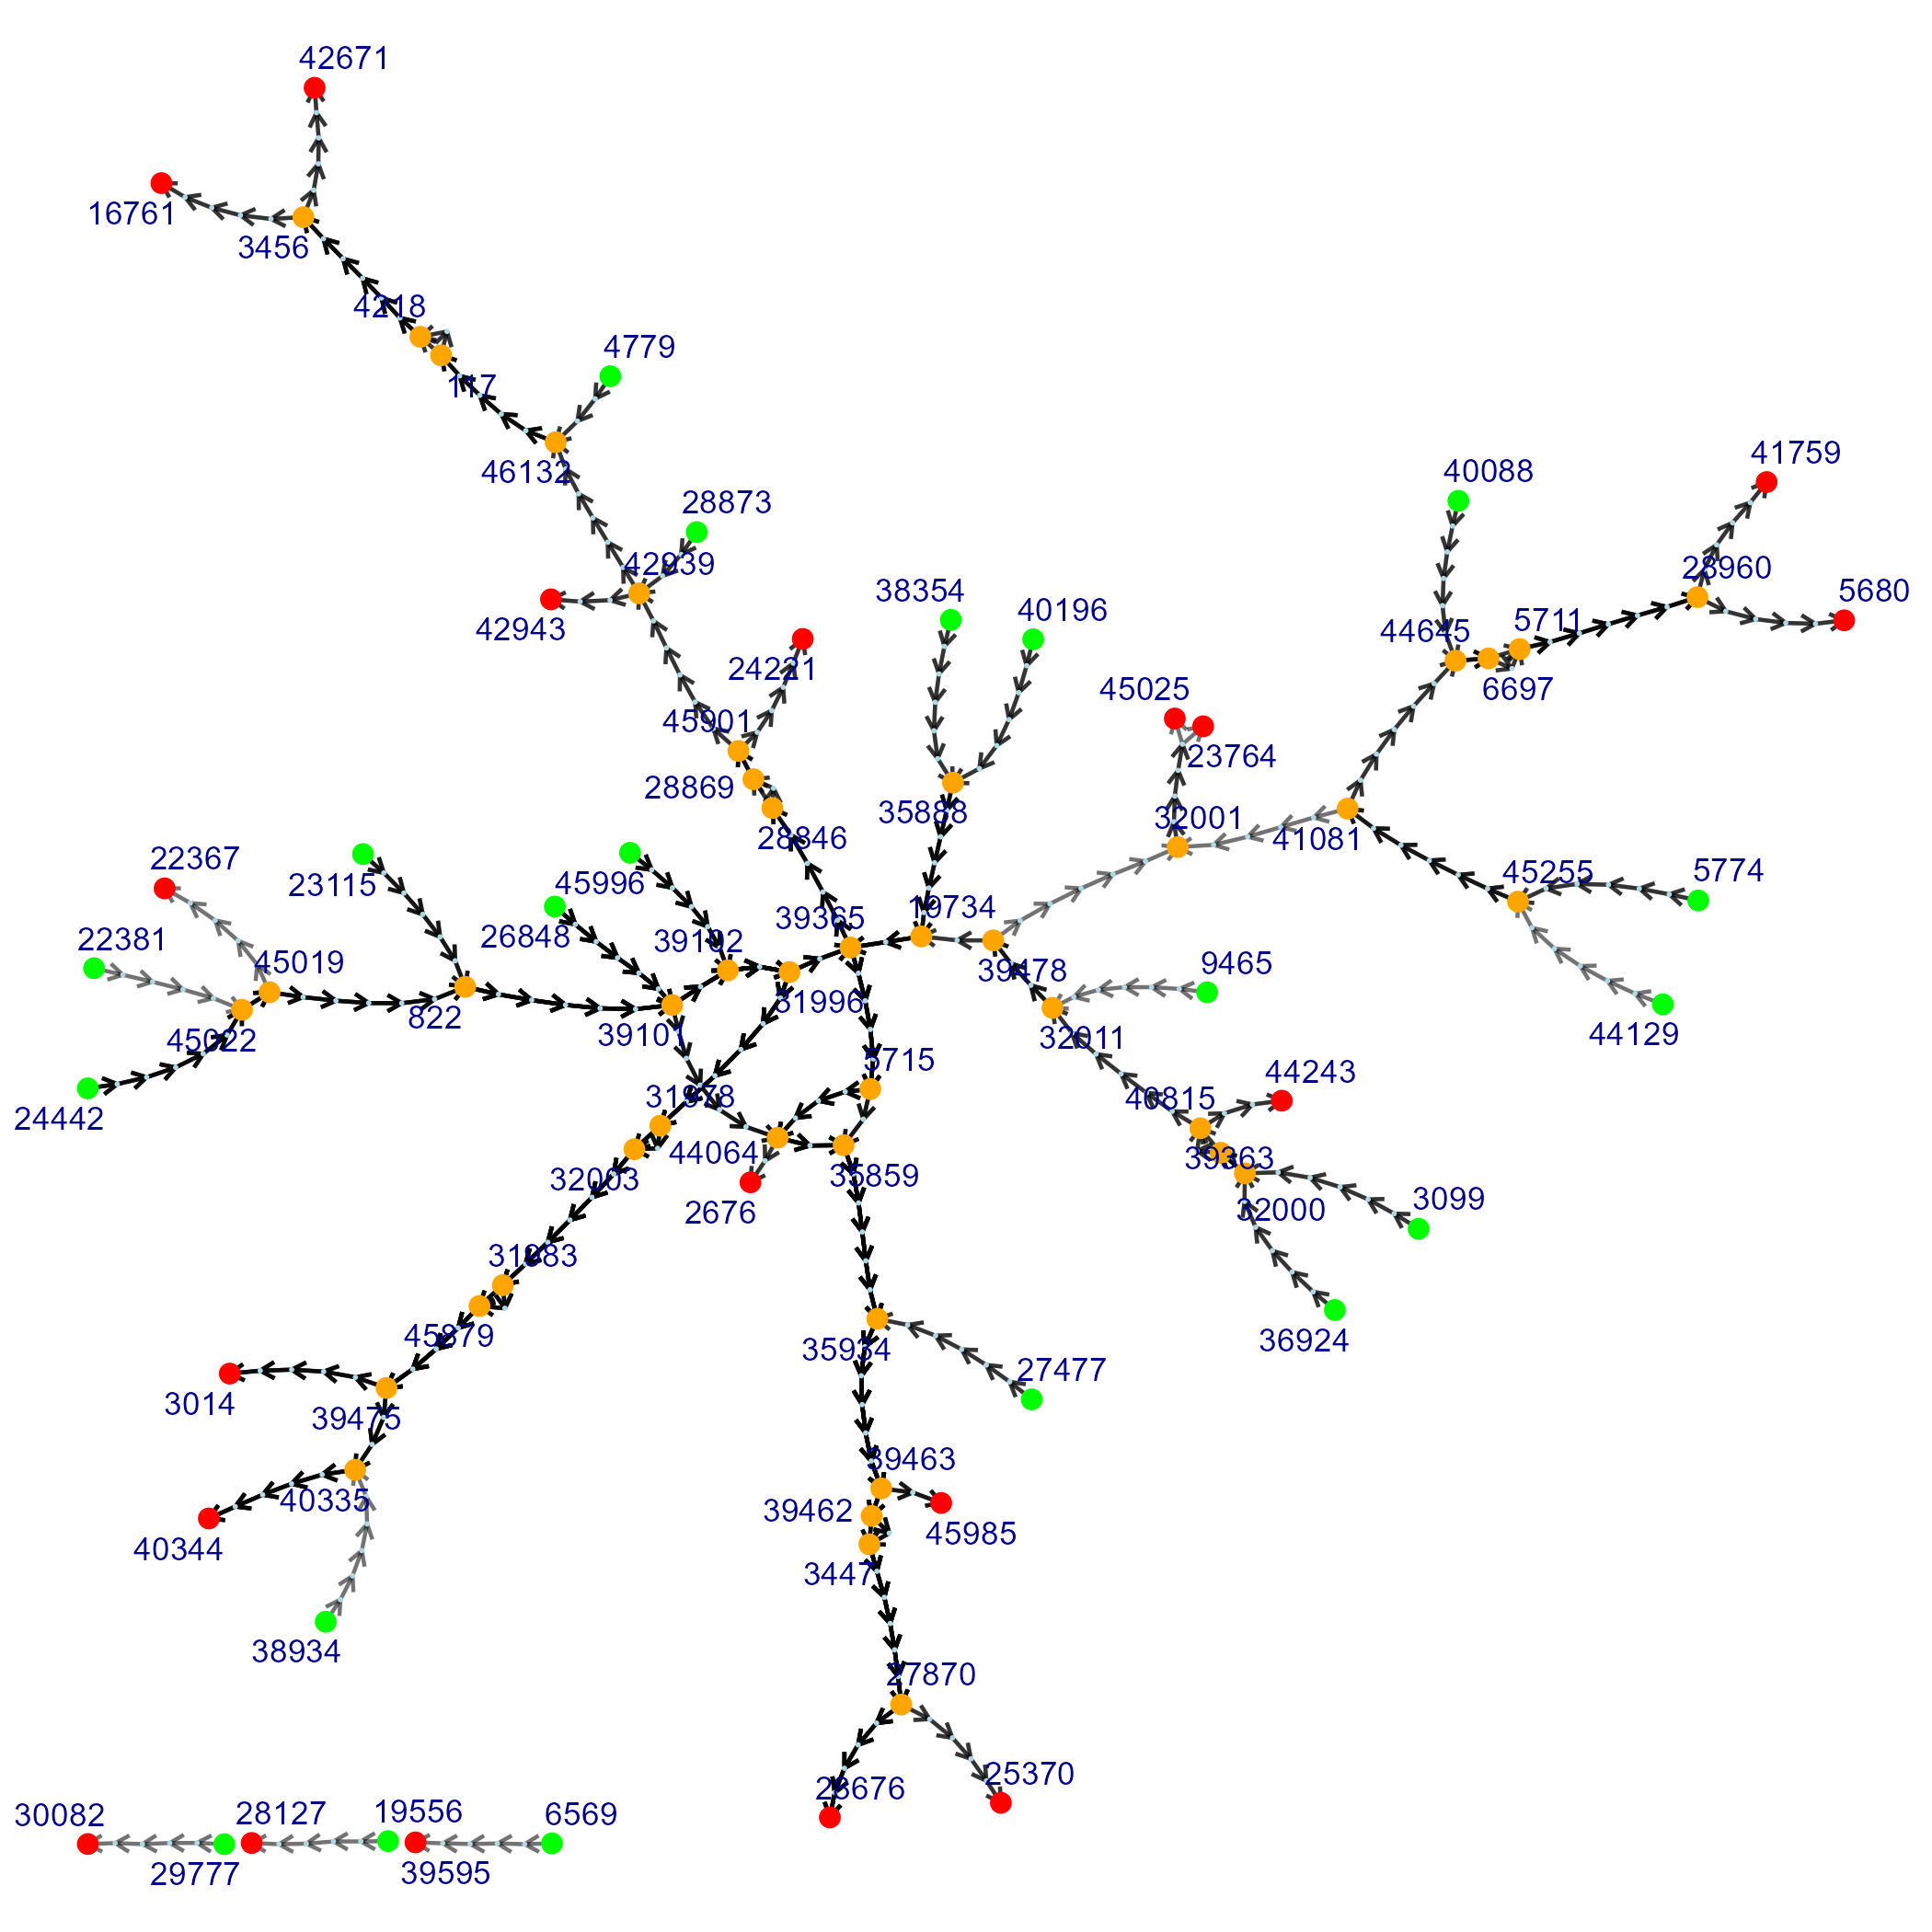
\includegraphics[width=\linewidth]{img/R_network.jpg}
    \caption{A simplified 20 trips network plot}
    \label{network_plot1}
\end{figure}

\section{Scheduled rides}
The main difference between scheduled rides and on-demand rides is that we do not know the route and still have the starting time, starting, and ending point.

The metric graph in section \ref{sec:Construction of the Metric graph} is not fully connected. For example, if we want to travel from $46132$ to $4779$, based on the figure \ref{network_plot1}, we have to use some edges in the opposite direction, although no recorded driver has done this before. We develop a ``two-way" metric graph by allowing some opposite-direction movements. The statistics of the opposite movements are fictional, predicted based on the data of traveling from the same starting edge to other edges. Use the example in \ref{sec:Construction of the Metric graph}, the fictional statistics of travel from $6541$ to $1$ should be the same as from $6541$ to $6494$. 

Another challenge in the connection $\times$ time bin dataset is that our data does not fully cover all time bins. We may not observe any drivers passing some edge in, say, EveningNight, and still need to predict the duration. We solve this problem by adding a Global time bin, which uses all records in the connection to calculate the statistics, and uses it when some time bin data is missing.

We use the route-finding algorithm by \cite{1970algorithm} in the igraph (\cite{igraph}) package. The routes are in ascending order by length, so we can then calculate the expected travel time or simulate them.

\section{Membership}\label{sec:membership}
Although we have discussed some technologies in Section \ref{sec:Construction of the Metric graph}, finding all paths starting and ending at given points (see equations \ref{eq:scheduled-price} and \ref{eq:membership-price}) is too time-consuming. So, we introduced some sample methods to generate "similar" routes. These methods can also be helpful for membership pricing.
\subsection{Route Sampling}\label{sec:case-study}
In this subsection, we will discuss a simple method for membership pricing that may useful for some routine trips. Like going from the users' home to their work place and going back once per day. Under this setting, only some users' history trips and distance of the trips are known. For simplicity, we assume the interest rate to be $0.$ The membership pricing process for $r$ future days is as follow.

\begin{enumerate}
    \item If the users' trip distance from the users' home to their work place and going back distance are similar, we similar two trips per day. Otherwise, use this process twice for two distances.
    \item Define the distance range. If the user has only one record, we use $90\%\sim110\%$ of the distance. Otherwise, we use the minimum to maximum distance in the record.
    \item Depend on the user record, sample $r$ or $2r$ real trips in the global trip dataset, with the trip distance within the given range.
    \item Use the prediction process in \cite{elmasri2020predictive} to find expectations and variances of the sampled trip time.
    \item Use the expectations and variances to calculate the premium and expected trip price.
    \item Add all expands up and devide by $r$ to find the daily price.
\end{enumerate}


We selected $14$ trips that go either from edge $6346$ to $14800$, or from $14800$ to $6346$. The distance, depending on the specific route, is around $16500$ meters or $7000$ meters, with exactly the same probability. We assume that base on the trip ID, the smallest two trips are take place in one day and we observed (their distance are $16444.9$ and $6813,2$ meteres), and the remaining $12$ trips is a users' future commuting trip that needs a weekly membership. 



\section{Out-of-sample simulation}
 Now, we consider a trip number membership. Assume we observed some trips and need to simulate $r$ new trips. The sampling process is as follow.

\begin{enumerate}

        \item Randomly sample with replacement $r$ edge numbers and start times from the user's history data.
        \item Convert start times to corresponding {time bins}.
        \item For each edge in the simulated trip:
        \begin{itemize}
            \item Select edges from historical records within the matching time bin.
            \item Use weighted probabilities based on recorded edge frequencies.
            \item Record the distance in meters for each fictional trip; we need time and distance to find the trip cost.
        \end{itemize}
        \item Predict/simulate the travel time of the new fictional trip data. The prediction process is available from \cite{elmasri2020predictive}.
        \item Calculate price information for each simulated trip:
        \begin{itemize}
            \item Use the predicted travel time to calculate the ``expected" trip cost ($P_{expected}$).
            \item Use the simulated travel time to calculate the ``real" trip cost ($P_{real}$).
            \item The predicting process also included the variance of the trip time, so use the variance and expectation to calculate the premium (denote as $R$, the formula is \ref{eq:european-knock-in}).
        \end{itemize}
        \item The price of r trips membership would be the sum of all trips' $P_{expected}$ and $R$.

    
\end{enumerate}

If we wish to have protection against potential abusive loss or have a pressure test, we could limit the edge number sampling quantile of some trips (like only sampling from the longest 50\% trips for 10\% of the trips). Here, the minimum quantile could be interpreted as severity denoted as $s$, and the proportion of trips that applied the limited quantile is $\lambda$. 

Formally, if we wish to simulate $r$ trips for the user under a pressured state. Then we modify the first step of the sampling process above to:

\begin{enumerate}
        \item Randomly sample with replacement:
            \begin{itemize}
                \item $r-\lceil r*\lambda\rceil$ edge numbers and start times from the user's history data
                \item $\lceil r*\lambda\rceil$ edge numbers and start times from $s$ to $1$ quantile of the global data
            \end{itemize}
\end{enumerate}

In the following table, we make a pressure test simulation. Here we assume the interest rate to be zero, and $K$ equal to the ``expected" price. To make the results reproducible, we choose the seed $12345.$ Every number in the table was calculated with the following process:
\begin{enumerate}
    \item Empty the memory and start a new session, set the seed to be $12345.$
    \item Randomly sample $1000$ trips to make the test set, and use the remaining trip data as the training set.
    \item Sample $1000$ fictional trips for both normal and pressured states. Record the abuse ratio and $\lambda$. Find the corresponding $P_{i,expected, normal}$, $R_{i,normal}$, and $P_{i,real, pressure}$ for $i\in 1,2,3,...,1000$.
    \item The income (price charged to user) per trip is equal to: income = $\frac{1}{1000}\sum_{i=1}^{1000}P_{i,expected, normal}+R_{i, normal}$. 
    \item The pressure test result for trip $i$, as percentage return, at given severity and $\lambda$ should be equal to: return$_i$ = $({\text{income} - P_{real, pressure}}) / {\text{income}}\times 100\%.$
    \item In Table 1, the numbers are the average of the pressure test results. $\frac{1}{1000}\sum_{i=1}^{1000}$return$_i$ In Table 2, the numbers are the estimated standard deviation of the average return. The formula is $\frac{1}{\sqrt{1000}}\sqrt{\frac{1}{999}\sum_{i=1}^{1000}(\text{return}_i-\frac{1}{1000}\sum_{i=j}^{1000}\text{return}_j)^2}$.
\end{enumerate}




We found that using the seed $12345,$ the income is $\sim\$$25.8 per trip. Compared to the real cost calculated based on the test set, the average return is $\sim$6.45\%. Our pressure test results are presented in the following table.

\begin{figure}
    \centering
    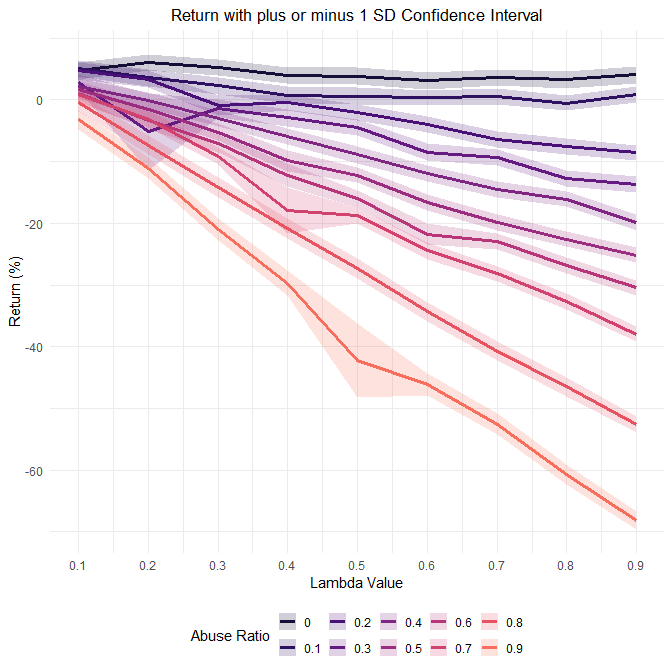
\includegraphics[width=1\linewidth]{sensitive_test.png}
    \caption{Sensitive test result}
    \label{sensitive_test}
\end{figure}

\begin{table}[ht]
\centering
\caption{\textbf{\% Average Return at Different Pressure Settings}}
\begin{tabular}{l | *{9}{r}}
\toprule
\multicolumn{1}{c|}{\footnotesize{s}} & \multicolumn{9}{c}{$\lambda$} \\ 
 \cmidrule(lr){2-10} 
 {\footnotesize }& 0.1    & 0.2     & 0.3      & 0.4      & 0.5      & 0.6       & 0.7       & 0.8       & 0.9       \\
\midrule
0    & 4.76473 & 6.06275 & 5.24833  & 3.98635 & 3.87400  & 3.09900  & 3.60528  & 3.26188    & 4.09142 \\
0.1  & 5.04958 & 3.56516 & 2.26873  & 0.80165   & 0.63042 & 0.32567  & 0.53412  & -0.52581  & 0.82856  \\
0.2  & 4.71596 & 3.39372 & -0.91624 & -0.39472 & -2.10115 & -4.01964  & -6.47903 & -7.55500  & -8.57397  \\
0.3  & 2.84991 & -5.16797 & -1.39935 & -2.91047 & -4.50369 & -8.44136  & -9.31158  & -12.7652  & -13.7512  \\
0.4  & 2.18284 & -0.08512 & -2.96998 & -5.94576 & -8.90094 & -11.9264  & -14.5637  & -16.0634  & -19.8439 \\
0.5  & 1.6512 & -1.56226  & -5.21708 & -9.86191 & -12.1673 & -16.6746  & -19.7869  & -22.5785 & -25.1562 \\
0.6  & 1.06770 & -3.31014 & -7.03568 & -12.1923 & -16.0381 & -21.7277  & -22.9624 & -26.8280  & -30.4616  \\
0.7  & 0.87888 & -3.11505 & -9.12327 & -17.9295 & -18.7089 & -24.4353  & -28.1903  & -32.6669  & -37.9605  \\
0.8  & -0.44871 & -7.32223 & -14.2363 & -20.8831 & -27.3653 & -34.3353  & -40.7257  & -46.5174  & -52.6035  \\
0.9  & -3.21756 & -11.0714 & -21.0129 & -29.6657 & -42.2083 & -46.1438  & -52.5469 & -60.6900  & -68.1493  \\
\bottomrule

\end{tabular}
\end{table}


\begin{table}[ht]
\centering
\caption{\textbf{\% Standard deviation of Average Return at Different Pressure Settings}}
\begin{tabular}{l | *{9}{r}}
\toprule
\multicolumn{1}{c|}{\footnotesize{s}} & \multicolumn{9}{c}{$\lambda$} \\ 
 \cmidrule(lr){2-10} 
 {\footnotesize }& 0.1    & 0.2     & 0.3      & 0.4      & 0.5      & 0.6       & 0.7       & 0.8       & 0.9       \\
\midrule
0 & 1.38 & 1.32 & 1.35 & 1.35 & 1.35 & 1.38 & 1.33 & 1.37 & 1.39 \\
0.1 & 1.31 & 1.35 & 1.34 & 1.31 & 1.33 & 1.27 & 1.25 & 1.25 & 1.27 \\
0.2 & 1.32 & 1.30 & 1.58 & 1.29 & 1.29 & 1.31 & 1.29 & 1.30 & 1.26 \\
0.3 & 1.35 & 6.28 & 1.44 & 1.33 & 1.26 & 1.34 & 1.30 & 1.29 & 1.27 \\
0.4 & 1.35 & 1.35 & 1.34 & 1.33 & 1.31 & 1.35 & 1.28 & 1.18 & 1.23 \\
0.5 & 1.38 & 1.37 & 1.39 & 1.72 & 1.27 & 1.31 & 1.29 & 1.25 & 1.17 \\
\bottomrule

\end{tabular}
\end{table}

From the table, we notice that when both the abuse ratio and $\lambda$ are positive, the returns are decreasing monotonically in most cases. This property aligns with our theory, validating the test methodology.

The return pressure test outcomes show that when the abuse ratio is zero,  positive returns persist even at elevated $\lambda$ values (e.g., 4.09\% at $\lambda=0.9$). When $\lambda$ is low, like $0.1$, the return also stays positive as the abuse ratio reaches $0.7$. The positive numbers are located in a curse region, indicates the multiplication relationship between the overall stress and the two risk variables. The return rates exhibit remarkable deterioration as both parameters increase at the same time. For instance, a return rate of $-16.67\%$ at $0.5,\,0.6$ for the abuse ratio and $\lambda$ respectively; during extreme pressure scenarios (abuse ratio$=0.9$, $\lambda=0.9$), the returns are down to $-68.1493\%$, warning of the risk in the negative tail. While under moderate pressure (e.g., abuse ratio$\leq0.5$,$\lambda\leq0.5$), most abuse ratios correspond to manageable return levels, indicating systemic resilience under pressure conditions.

In the standard deviation(SD) table, most scenarios exhibit moderate standard deviations ($40\sim50\%$). When we compare the data horizontally from left to right, the volatility gradually increases and then falls back. This pattern is quite reasonable because the increase $\lambda$ will mix two different distributions with different weight, and the standard deviation would increase when the large and small returns are spread more evenly. We also notice that our $\pi_{pop}$ dataset included some extremely long trips. Therefore, if the sample process included these trips, the return would be significantly low and the standard deviation would be very large. For example, when $\lambda=0.2$ and abuse ration = $0.3.$ However, when abuse ration is low, this unfortunate event has a very low probability; also notice that when the abuse ratio is high, the return would not be lower than the return of the next level (when $\lambda=0.4$ abuse ration = $0.7$, and $\lambda=0.5$ and abuse ration = $0.9)$. This simulation result emphasized the robustness of the pricing strategy, providing an actionable methodology to calculate return expectations and modify risk tolerance.

\section{Notations}


\begin{longtable}{|c|c|l|}
\hline
\textbf{Variables} & \textbf{Section}  & \textbf{Meaning}\\
\hline
\endfirsthead
\hline
\textbf{Variables} & \textbf{Section}  & \textbf{Meaning}\\
\hline
\endhead
\hline
\endfoot
\hline
\endlastfoot
\(B\) & \ref{sec:sampler} & The time bin set\\
\(B_{s}\) & \ref{sec:traveltime-process} & Brownian process\\
\(C_{(\cdot)}\) & \ref{sec:cyclostationary}, \ref{sec:pricing-main}, \ref{sec:upfront}, \ref{sec:profit analysis} & (an absolute constant in \ref{sec:cyclostationary})(a continuous function in \ref{sec:metric-graph})Pricing coefficients\\
\(E,\,E_{(\cdot)}\) & \ref{sec:sampler} & Connection set and Edge statistics \\
\(\cE\) & \ref{sec:background} & Edge set \\
\(\cG\) & \ref{sec:background}, \ref{sec:pricing-main}, \ref{sec:complex-pricing}, \ref{sec:sampler} & Metric graph \\
\(K\) & \ref{sec:introduction}, \ref{sec:pricing-main},  \ref{sec:upfront}, \ref{sec:complex-pricing}, \ref{sec:profit analysis}, \ref{sec:membership} & Strike price of the membership\\
\(L_2\)&\ref{sec:metric-graph} & \\
\(M\) & \ref{sec:complex-pricing} & Maximum number of rides of a membership \\
\(\mathbb{N}\)& \ref{sec:complex-pricing} & Natrual number set\\
\(N(\mu,\sigma^2)\) & \ref{sec:introduction},\ref{sec:traveltime-process} & A normal distribution with mean $\mu$ and variance $\sigma^2$\\
\(\cN(\cG,X)\) & \ref{sec:traveltime-process} & Transportation network\\
\(P_{(\cdot)}\) & \ref{sec:introduction}, \ref{sec:pricing-main}& Price of a ride \\
\(R_{(\cdot)}(\cdots)\) & \ref{sec:upfront}, \ref{sec:complex-pricing} & Premium price (maximum number of rides of a membership in \ref{sec:complex-pricing})\\
\(\R_+\) & \ref{sec:traveltime-process} & Positive real number set \\
\(T_{(\cdot)}\) & \ref{sec:introduction}, \ref{sec:cyclostationary}, \ref{sec:complex-pricing}, \ref{sec:profit analysis} & The stop time of a trip or a membership \\
\(\mathcal{T}^{(\cdot)}_{(\cdot)}\) & \ref{sec:traveltime-process}, \ref{sec:pricing-main}, \ref{sec:complex-pricing}, \ref{sec:travel time sampling}, \ref{sec:discussion}& Travel time up to a location\\
\(U_{(\cdot)}\) & \ref{sec:travel time sampling}, \ref{sec:discussion} & Some uniform random variables \\
\(\mathcal{V}\) & \ref{sec:metric-graph} & Set of vertices\\
\(X\) & \ref{sec:cyclostationary}, \ref{sec:traveltime-process}& A spatio-temporal process \\
\(Z_{(\cdot)}\) & \ref{sec:travel time sampling} & Some normal random variables \\
\(b\) & \ref{sec:route sampling} & A time bin\\
\(d_{(\cdot)}\) & \ref{sec:upfront}, \ref{sec:profit analysis} & Intermediate parameters to find premium\\
\(e_{(\cdot)}\)& \ref{sec:background}, \ref{sec:pricing-main}, \ref{sec:upfront}, \ref{sec:complex-pricing}, \ref{sec:sampler}, \ref{sec:profit analysis}, \ref{sec:discussion}
& An edge, (natural constant in \ref{sec:pricing-main}, \ref{sec:upfront}, \ref{sec:complex-pricing}, \ref{sec:profit analysis}) \\
\(i\) & \ref{sec:pricing-main}, \ref{sec:profit analysis} & Interest rate \\
\(l_{(\cdot)}\) & \ref{sec:background} & A length \\
\(m_{(\cdot)}(t,s)\) & \ref{sec:cyclostationary}, \ref{sec:traveltime-process}, \ref{sec:sampler}, \ref{sec:discussion}& Expected travel time.\\
\(n_{(\cdot)}\) & \ref{sec:background}, \ref{sec:sampler} & Number of something \\
\(r\) & \ref{sec:upfront}, \ref{sec:complex-pricing}, \ref{sec:profit analysis} & Risk free interest rate \\
\(s\) & \ref{sec:background}, \ref{sec:pricing-main}, \ref{sec:upfront}, \ref{sec:complex-pricing} & Position \\
\(t_{(\cdot)}\) & \ref{sec:introduction}, \ref{sec:background}, \ref{sec:pricing-main}, \ref{sec:upfront}, \ref{sec:complex-pricing}, \ref{sec:travel time sampling}, \ref{sec:profit analysis}, \ref{sec:discussion} & Time \\
\(x\) & \ref{sec:background} & The distance to the beginning of an edge\\
\(\alpha\) & \ref{sec:traveltime-process} & Expectation parameter of the stochastic process \\
\(\beta\) & \ref{sec:traveltime-process} & Variance parameter of the stochastic process  \\
\(\delta_{(\cdot)}\) & \ref{sec:background}, \ref{sec:pricing-main}, \ref{sec:profit analysis} & The distance of a shortest route. \\
\(\epsilon_{(\cdot)}(t,s)\) & \ref{sec:cyclostationary}, \ref{sec:traveltime-process} & Residual of the travel time\\
\(\zeta\) & \ref{sec:upfront}, \ref{sec:route sampling}, \ref{sec:profit analysis} & The minimum threshold for the guarantee/edge similarity\\
\(\eta\) & \ref{sec:traveltime-process} & A strictly positive, universal residual parameter \\
\(\mu\) & \ref{sec:introduction}, \ref{sec:background} & Mean of a distribution\\
\(\widehat{\mu}\) & \ref{sec:travel time sampling} & The global sample mean \\
\(\xi\) & \ref{sec:traveltime-process}, \ref{sec:travel time sampling}, \ref{sec:fedelity} & (Some absolute constant in \ref{sec:traveltime-process}), the correlation coefficient\\
\(\pi(\cdots)\) &\ref{sec:background}, \ref{sec:pricing-main}, \ref{sec:complex-pricing} & Probability of selecting a route \\
\(\Pi(\cdot,\cdot)\) & \ref{sec:background}, \ref{sec:complex-pricing} & Set of all routes between two edges. \\
\(\rho_{(\cdot)}\) & \ref{sec:introduction}, \ref{sec:background}, \ref{sec:pricing-main}, \ref{sec:upfront}, \ref{sec:complex-pricing}, \ref{sec:route sampling}, \ref{sec:profit analysis}, \ref{sec:on demand simulation} & A route \\
\(\sigma_{(\cdot)}\) & \ref{sec:introduction}, \ref{sec:background}, \ref{sec:sampler}, \ref{sec:fedelity}, \ref{sec:discussion} & Standard deviation/covariance of a distribution\\
\(\varsigma(t,u,s)\) & \ref{sec:cyclostationary} & Correlation of travel duration between connected edges.\\
\(\Sigma\) & \ref{sec:travel time sampling}, \ref{sec:fedelity} & The variance matrix of some multivariate distribution \\
\(\T_{e^-}\) & \ref{sec:traveltime-process} & Random
arrival time at some edge\\
\(\phi\) & \ref{sec:upfront}, \ref{sec:profit analysis} & Standard normal probability density function\\
\(\Phi\) & \ref{sec:upfront}, \ref{sec:travel time sampling}, \ref{sec:profit analysis}, \ref{sec:discussion} & Standard normal cumulative density function \\
\end{longtable}

\end{appendices}
\end{document}